\documentclass{CU_DH} % Thesis class with hyperref
%\documentclass{thesis}        % old CU thesis class
\usepackage[pdftex]{graphicx}  % for figures
%\usepackage[section]{placeins} % keep floats in the same section. 
\usepackage{lipsum}            % for filler text in latin
\usepackage{color}             % for color.
\usepackage{amsmath}

\newif\ifprinted
\printedtrue
%\printedfalse
\ifprinted
\usepackage[colorlinks=true,linkcolor=black,urlcolor=black,
            citecolor=black]{hyperref} 
\else
\usepackage[colorlinks=true,linkcolor=blue,urlcolor=blue,
            citecolor=blue]{hyperref} 
\fi
\usepackage{enumitem}         % better lists 
\usepackage{subcaption}       % multi-panel figures 
\usepackage{longtable}        % multi-page tables 
\usepackage[skip=4pt]{caption} % smaller gap between figure and caption

 % gap between bottom of caption and text. Give tex a little flexibility.
%\setlength{\intextsep}{0pt plus 4pt}
%\setlength{\textfloatsep}{12.0pt plus 2.4pt minus 2.4pt}

\def \FigPath {../} % DEFINE PATH TO FIGURES %

% use these to include only one chapter, for quick compiles
%\includeonly{Abbreviations}
%\includeonly{Outline}
\includeonly{Introduction}
%\includeonly{Experiment}
%\includeonly{ATI}
%\includeonly{PEI}
%\includeonly{Shock}
%\includeonly{Conclusion}
%\includeonly{Appendix}
%\includeonly{AppendixATI}
%\includeonly{AppendixPEI}
%\includeonly{AppendixShock}







% % % % %For quotes at the start of chapters
%see: http://tex.stackexchange.com/questions/13756/quote-environment-with-reference-at-the-end-right
\def\signed #1{{\leavevmode\unskip\nobreak\hfil\penalty50\hskip2em
		\hbox{}\nobreak\hfil --#1%
		\parfillskip=0pt \finalhyphendemerits=0 \endgraf}}

\newsavebox\mybox
\newenvironment{aquote}[1]
{\savebox\mybox{#1}\begin{quote}}
	{\signed{\usebox\mybox}\end{quote}}

% % % % % % % % % % % % % % %

% % % % % % % % % % % Now for some serious citation antics  
\usepackage[backend=bibtex,backref=true,natbib=false,style=numeric-comp,firstinits=true,url=false,doi=true,date=year,isbn=false,maxcitenames=20,maxbibnames=40,minbibnames=30,sorting=none]{biblatex}  

\DefineBibliographyStrings{english}{%
	backrefpage = {cited on page},
	backrefpages = {cited on pages},
}  

%get rid of the "in"			
\renewbibmacro{in:}{\ifentrytype{article}{}{\printtext{\bibstring{in}\intitlepunct}}}
\DeclareFieldFormat[article]{pages}{#1}%Remove "pp." before pages
\DeclareFieldFormat{journaltitle}{\textit{#1},} %italic journal
\DeclareFieldFormat[article,inbook,incollection,inproceedings,patent,thesis,unpublished]{title}{#1} %remove quoted from title
\DeclareFieldFormat[article]{date}{\textbf{#1}} %bold date

%Add parentheses to the issue number
\renewbibmacro*{volume+number+eid}{%
	\printfield{volume}%
	%  \setunit*{\adddot}% DELETED
	\setunit*{\addnbspace}% NEW (optional); there's also \addnbthinspace
	\printfield{number}%
	\setunit{\addcomma\space}%
	\printfield{eid}}
\DeclareFieldFormat[article]{number}{\mkbibparens{#1}}

%remove parentheses from the date
\renewbibmacro*{issue+date}{%
	\setunit{\addcomma\space}% NEW
	%  \printtext[parens]{% DELETED
	\iffieldundef{issue}
	{\usebibmacro{date}}
	{\printfield{issue}%
		\setunit*{\addspace}%
		%       \usebibmacro{date}}}% DELETED
		\usebibmacro{date}}% NEW
	\newunit}

%Make a command to cite with no square brackets:
\DeclareCiteCommand{\citeNoBrackets}%[\mkbibbrackets]
{\usebibmacro{cite:init}%
	\usebibmacro{prenote}}
{\usebibmacro{citeindex}%
	\usebibmacro{cite:comp}}
{}
{\usebibmacro{cite:dump}%
	\usebibmacro{postnote}}


%Use the URL if the DOI is not available.
%from: http://tex.stackexchange.com/questions/154864/biblatex-use-doi-only-if-there-is-no-url
\renewbibmacro*{doi+eprint+url}{%
  \iftoggle{bbx:doi}
    {\iffieldundef{doi}{\printfield{url}}{\printfield{doi}}}
	{}%
  \newunit\newblock
  \iftoggle{bbx:eprint}
	{\usebibmacro{eprint}}
	{}%
  \newunit\newblock
  \iftoggle{bbx:url}
	{\usebibmacro{url+urldate}}
	{}}

%Put the authors in beautiful small caps
%\renewcommand{\mkbibnamefirst}[1]{\textsc{#1}}
%\renewcommand{\mkbibnamelast}[1]{\textsc{#1}}
%\renewcommand{\mkbibnameprefix}[1]{\textsc{#1}}
%\renewcommand{\mkbibnameaffix}[1]{\textsc{#1}}

%\addbibresource{/Users/dcc2/Desktop/BIBFiles/111ColeThesisBIB.bib}
\addbibresource{111ColeThesisBIB.bib}
%\addbibresource{/Users/dcc2/Desktop/BIBFiles/fakefile.bib}

% % % % % % % % % % % % Okay, done with citations. Phew. That got crazy.

%Add a way to put quotes at the start of chapters:
\newenvironment{chapquote}[2][2em]
{\setlength{\@tempdima}{#1}%
	\def\chapquote@author{#2}%
	\parshape 1 \@tempdima \dimexpr\textwidth-2\@tempdima\relax%
	\itshape}
{\par\normalfont\hfill--\ \chapquote@author\hspace*{\@tempdima}\par\bigskip}
\makeatother

% % % % % % % % % % % % % % % % % % % % % % % % % % % % % %
%IMPORTANT: The Colorado thesis class file does not place figures (floats) well.
%This fixes two mistakes in the class file and places floats intellegently
% See http://robjhyndman.com/hyndsight/latex-floats/
% and http://mintaka.sdsu.edu/GF/bibliog/latex/floats.html
% General parameters, for ALL pages:
\renewcommand{\topfraction}{0.9}	% max fraction of floats at top
\renewcommand{\bottomfraction}{0.9}	% max fraction of floats at bottom
% Parameters for TEXT pages (not float pages):
\setcounter{topnumber}{2}       % Max number of floats on top
\setcounter{bottomnumber}{2}    % Max number of floats on bottom
\setcounter{totalnumber}{4}     % Max floats on page, 2 may work better
\setcounter{dbltopnumber}{2}    % for 2-column pages
\renewcommand{\dbltopfraction}{0.9}	% fit big float above 2-col. text
\renewcommand{\textfraction}{0.07}	% allow minimal text w. figs
% Parameters for FLOAT pages (not text pages):
\renewcommand{\floatpagefraction}{0.89}	% require fuller float pages
  % floatpagefraction MUST be less than topfraction 
\renewcommand{\dblfloatpagefraction}{0.7}	% require fuller float pages

%------------------------------------------------
% Preamble material
%------------------------------------------------

% % % % % % % % % % % % % % % % % %
\title{ThesisTitle}
\author{Daniel C.}{Cole}
% % % % % % % % % % % % % % % % % %

\otherdegrees{Other Degrees}

\degree{Doctor of Philosophy}		%  #1 {long descr.}
	{Ph.D., Physics}		%  #2 {short descr.}

\dept{Physics}			%  #1 {designation}
		{Physics}    	%  #2 {name}

\advisor{Dr.}				%  #1 {title}
	{Scott A. Diddams}			%  #2 {name}

\reader{Reader1}		%  2nd person to sign thesis
\readerThree{Reader2}
%\readerFour{David Jonas}
%\readerFive{David Jonas}

\abstract{  \OnePageChapter	% because it is very short
\lipsum [66]
	}


%\dedication[Dedication]{.......}


\acknowledgements{ %\OnePageChapter	% *MUST* BE ONLY ONE PAGE!
The work in this thesis would not have been possible... 
\begin{itemize}[leftmargin=*]
\item Acknowledgement line 1

\item Acknowledgement line 2


\end{itemize}
	}


%\ToCisShort	% use this only for 1-page Table of Contents

%\LoFisShort	% use this only for 1-page Table of Figures
% \emptyLoF	% use this if there is no List of Figures

%\LoTisShort	% use this only for 1-page Table of Tables
 \emptyLoT	% use this if there is no List of Tables
 

%%%%%%%%%%%%%%%%%%%%%%%%%%%%%%%%%%%%%%%%%%%%%%%%%%%%%%%%%%%%%%%%%
%%%%%%%%%%%%%%%         BEGIN DOCUMENT          %%%%%%%%%%%%%%%%%
%%%%%%%%%%%%%%%%%%%%%%%%%%%%%%%%%%%%%%%%%%%%%%%%%%%%%%%%%%%%%%%%%

\begin{document}

% % % % % % % % % % % % % % % % % % % % % % % % % % % % % %
% New Commands
%shortcut for non-italic units in math with a space in front:
\newcommand{\units}[1]{\ \mathrm{{#1}}} 

\newcommand{\wcmsq}{\units{W/cm^2}}     %shorcut for watts/cm^2
\newcommand{\ish}[1]{$\mathtt{\sim} {#1}$} %tilde for approximate value
\newcommand{\fixthis}{\marginpar{\textbf{\Large !!!}}}

%Shortcut for the copyright year for APS and ACS:
\newcommand{\ACS}[1]{\copyright {#1} American Chemical Society}
\newcommand{\APS}[1]{\copyright {#1} American Physical Society}

%Sometimes the parallel symbol looks weird, then use this one:
\newcommand{\myparallel}{{\mkern1mu\vphantom{\perp}\vrule depth 0pt\mkern2mu\vrule depth 0pt\mkern3mu}}

\newcommand{\micron}{$\mathrm{\mu m}$ }
\newcommand{\tio}{$\mathrm{TiO_2}$ } % just a shortcut for TiO2
\newcommand{\chem}[1]{$\mathrm{#1}$} % shortcut for chemical symbols


% % % % % % % % % % % % % % % % % % % % % % % % %
% this is the amateur bibliography. Use biblatex above
%\bibliographystyle{amsplain}
\pagenumbering{roman}
 \chapter*{List of Abbreviations}
 \label{ch:abbreviations}
 
% \begin{itemize}
% 	\item[] 



\begin{longtable}{l l}
	HRR & High repetition rate \\
	DC & Direct current \\
	RF & Radio frequency \\
	IM & Intensity modulation \\
	PM & Phase modulation \\
	HNLF & Highly-nonlinear fiber \\
	SMF & Single-mode fiber \\
	SLM & Spatial light modulator \\
	FWHM & Full-width at half-maximum \\
	SPM & Self-phase modulation \\
	DRO & Dielectric-resonator oscillator \\
%	ATI  & Above Threshold Ionization \\
%	ADK  & Ammosov, Delone, and Krainov \cite{Ammosov1986} -- an estimate of tunnel ionization rates\\
%	BBO  & Beta Barium Borate -- a nonlinear crystal \\
%	CCD  & Charge-Coupled Device -- the type of sensor in many digital cameras \\
%	CoM  & Center of Mass \\
%	CPA  & Chirped Pulse Amplification \\
%	DMA  & Differential Mobility Analyzer - A device that produces a size-selected aerosol\\
%	EUV  & Extreme Ultraviolet (light)\\
%	eV   & Electron Volt - unit of energy, $1 \units{eV} \approx 1.602\times 10^{-19} \units{J}$\\
%	FDTD & Finite-Difference Time-Domain -- a simulation method\\
%	HHG  & High-Harmonic Generation -- a method for producing EUV and SXR light\\
%	HYDRA& A radiation hydrodynamic code developed at Livermore National Lab\\
%	IR   & Infrared (light)\\
%	JILA & The Institute formerly known as the Joint Institute for Laboratory Astrophysics \\
%	MCP  & Microchannel Plate -- a detector of electrons, ions, and photons\\
%	OPA  & Optical Parametric Amplifier \\
%	PAD  & Photoelectron (or Photoion) Angular Distribution\\
%	PEI  & Plasma Explosion Imaging\\
%	PES  & Photoelectron Spectroscopy\\
%	psig & pounds per square inch gauge -- a unit of pressure in excess of atmospheric pressure \\
%	PSW  & Plane Spherical Wave -- a model for SFI presented in this thesis\\
%	PVP  & Polyvinylpyrrolidone  -- an organic compound\\ 
%	SFI  & Strong Field Ionization \\
%	SXR  & Soft X-ray \\
%	TDSE & Time-Dependent Schr\"{o}dinger Equation\\
%	ToF  & Time of Flight \\
%	UV   & Ultraviolet\\
%	VMI  & Velocity Map Imaging \\
%	VMIS & Velocity Map Imaging Spectrometer\\
\end{longtable}
 
 	
 	
% \end{itemize}
% \chapter{Outline}\label{chap:outline}

\pagenumbering{arabic}
 \chapter{Introduction}
\label{chap:introduction}

The optical frequency comb is a versatile tool for science and technology. Its invention two decades ago initiated a revolution in precision measurement by dramatically improving the resolution with which we can conveniently measure time and frequency \cite{Diddams2000,Jones2000,Udem2002,Hall2006,Hansch2006}. This revolution was brought about by advancements in nonlinear optics \cite{Ranka2000} that enabled the realization of a simple scheme by which the hundreds-of-terahertz-scale optical frequencies of a modelocked laser could be measured electronically, and was facilitated by the development of high performing solid-state femtosecond laser technology such as the Ti:sapphire laser. Since their introduction, optical frequency combs have found important roles in a range of experiments and applications, including the first demonstration of an optical atomic clock \cite{Diddams2001}, systems for ultra-low-noise microwave synthesis \cite{McFerran2005,Fortier2011}, broadband spectroscopy applications \cite{Diddams2007,Coddington2016}, optical arbitrary waveform generation \cite{Cundiff2010}, and stable long-term calibration of astronomical spectrographs for exoplanet detection \cite{Steinmetz2008}. Further development of the technology beyond the first stabilization of the Ti:sapphire laser that heralded the frequency comb's arrival has enabled combs to reach applications across many wavelength bands \cite{Washburn2004a,Gohle2005b,Diddams2010,Faist2016}. The technology is reaching maturity, and frequency combs have been commercially available for some time.

In the last decade, methods for generating optical frequency combs without a modelocked laser have emerged. These new frequency combs come with higher repetition rates and lower fundamental size, weight, and power (SWAP) requirements. Higher repetition rates make them particularly attractive for applications where high power per comb mode, individual accessibility of comb modes, and fast acquisition times are desired; these applications include arbitrary microwave and optical waveform generation, telecommunications, and broadband, temporally-resolved spectroscopy. The lower SWAP requirements of these combs suggest the tantalizing possibility that they could be used in these and other applications outside the laboratory. These combs present a promising route towards truly portable and robust frequency comb technology, which would continue to drive forward the revolution that was initiated some twenty years ago. There remains much work to be done, however, to develop these combs that are based on continuous-wave lasers to the level of technological maturity that has been reached by modelocked-laser-based combs.

%begun to suggest new ways to bring their capabilities to applications outside the controlled environment of the research laboratory.

%These combs are beginning, enabling e.g. direct optical frequency synthesis on a chip \cite{Spencer2018}.

%which could well lead to a second revolutionMoreover, these combs come with lower fundamental size, weight, and power (SWAP) requirements, which will enable them to provide the features that make modelocked-laser-based combs attractive in a more portable package. 

This thesis focuses on these new frequency combs, with several related, discrete areas of focus. The bulk of the thesis covers microresonator-based frequency combs (microcombs), and especially the nonlinear dynamics involved in the generation of these frequency combs via the Kerr nonlinearity. An introduction to this field is provided in Chapter \ref{chap:microresonators}. Chapters \ref{chap:PMPumping}-\ref{FPLLE} describe advancements in the field, and Chapter \ref{chap:Conclusion} provides a brief summary and a discussion of avenues for further research on this topic. Then, Chapter \ref{chap:EOMCombs} presents a second method for generating a high-repetition-rate frequency comb without modelocking that is based on active modulation of a CW seed laser and subsequent nonlinear spectral broadening. The first self-referencing of a comb of this type is described, and a proof-of-principle application to the generation of low-noise microwaves is discussed. An outlook for further development of this type of comb is presented. Finally, in Chapter \ref{chap:PulsePicking}, I present experimental and theoretical investigations of repetition-rate reduction of frequency combs via pulse gating, which may prove useful for adapting low-SWAP combs and their intrinsically high repetition rates to some applications as the technology continues to develop. 

In the remainder of this chapter, I discuss the basic properties of frequency combs and explain how the optical frequencies making up a comb can be fully determined by electronics operating with gigahertz-scale bandwidths.

\section{Optical frequency combs}

An optical frequency comb is obtained by fully stabilizing the spectrum of an optical pulse train. The first frequency combs came about through full frequency-stabilization of modelocked lasers; this thesis focuses on frequency combs with pulse trains generated through other means.

\subsection{Optical pulse trains and their spectra}

In the time domain, a frequency comb consists of a train of uniformly spaced optical pulses arriving at the pulse train's repetition rate $f_{rep}$, which within the growing space of frequency comb technology is between $\sim$10 MHz and $\sim$1 THz; the combs discussed in this thesis have repetition rates between 10 GHz and 30 GHz. In most implementations the pulses are very short compared to the repetition period $T=1/f_{rep}$, with durations on the order of 100 fs. In the frequency domain, the comb consists of a set of modes that are spaced by $f_{rep}$ in frequency and that have amplitudes determined by an overall spectral envelope centered at the optical carrier frequency $\nu_c$ ($\sim$193 THz in this thesis), with bandwidth inversely related to the temporal duration of the pulses. The usual description of a frequency comb, which is natural for modelocked-laser-based combs that are not derived from a CW laser, gives the frequencies of the comb modes as 
\begin{equation}
\nu_n=nf_{rep}+f_0, \label{eq:combfreqsold}
\end{equation} 
where $n\sim \nu_c/f_{rep}$ for the optical modes that make up the comb and $f_0$ is the carrier-envelope offset frequency, which may be defined to be between $0$ and $f_{rep}$. The offset frequency results from the pulse-to-pulse evolution of the carrier wave underneath the temporal intensity envelope of the pulses due to a difference in group and phase velocities. An equivalent representation of the frequencies of the comb that is more natural for frequency combs directly derived from a CW laser, as described in this thesis, is
\begin{equation}
\nu_\mu=\nu_c+\mu f_{rep}, \label{eq:combfreqsnew}
\end{equation} 
where $\nu_c$ is the frequency of the CW laser, the `pump' or `seed' laser, from which the frequency comb is derived and $\mu$ is a pump-referenced mode number, in contrast with the zero-referenced mode number $n$ of Eq. \ref{eq:combfreqsold}. Now the carrier-envelope offset frequency $f_0$ is found in the difference between $\nu_c$ and the closest harmonic of $f_{rep}$: $f_0=\nu_c-N f_{rep}$, where $N$ is the largest integer such that $f_0>0$. Fig. \ref{fig:CombBasics} depicts the properties of a frequency comb in the time domain and the frequency domain.

\begin{figure}[htpb]
	\begin{center}
		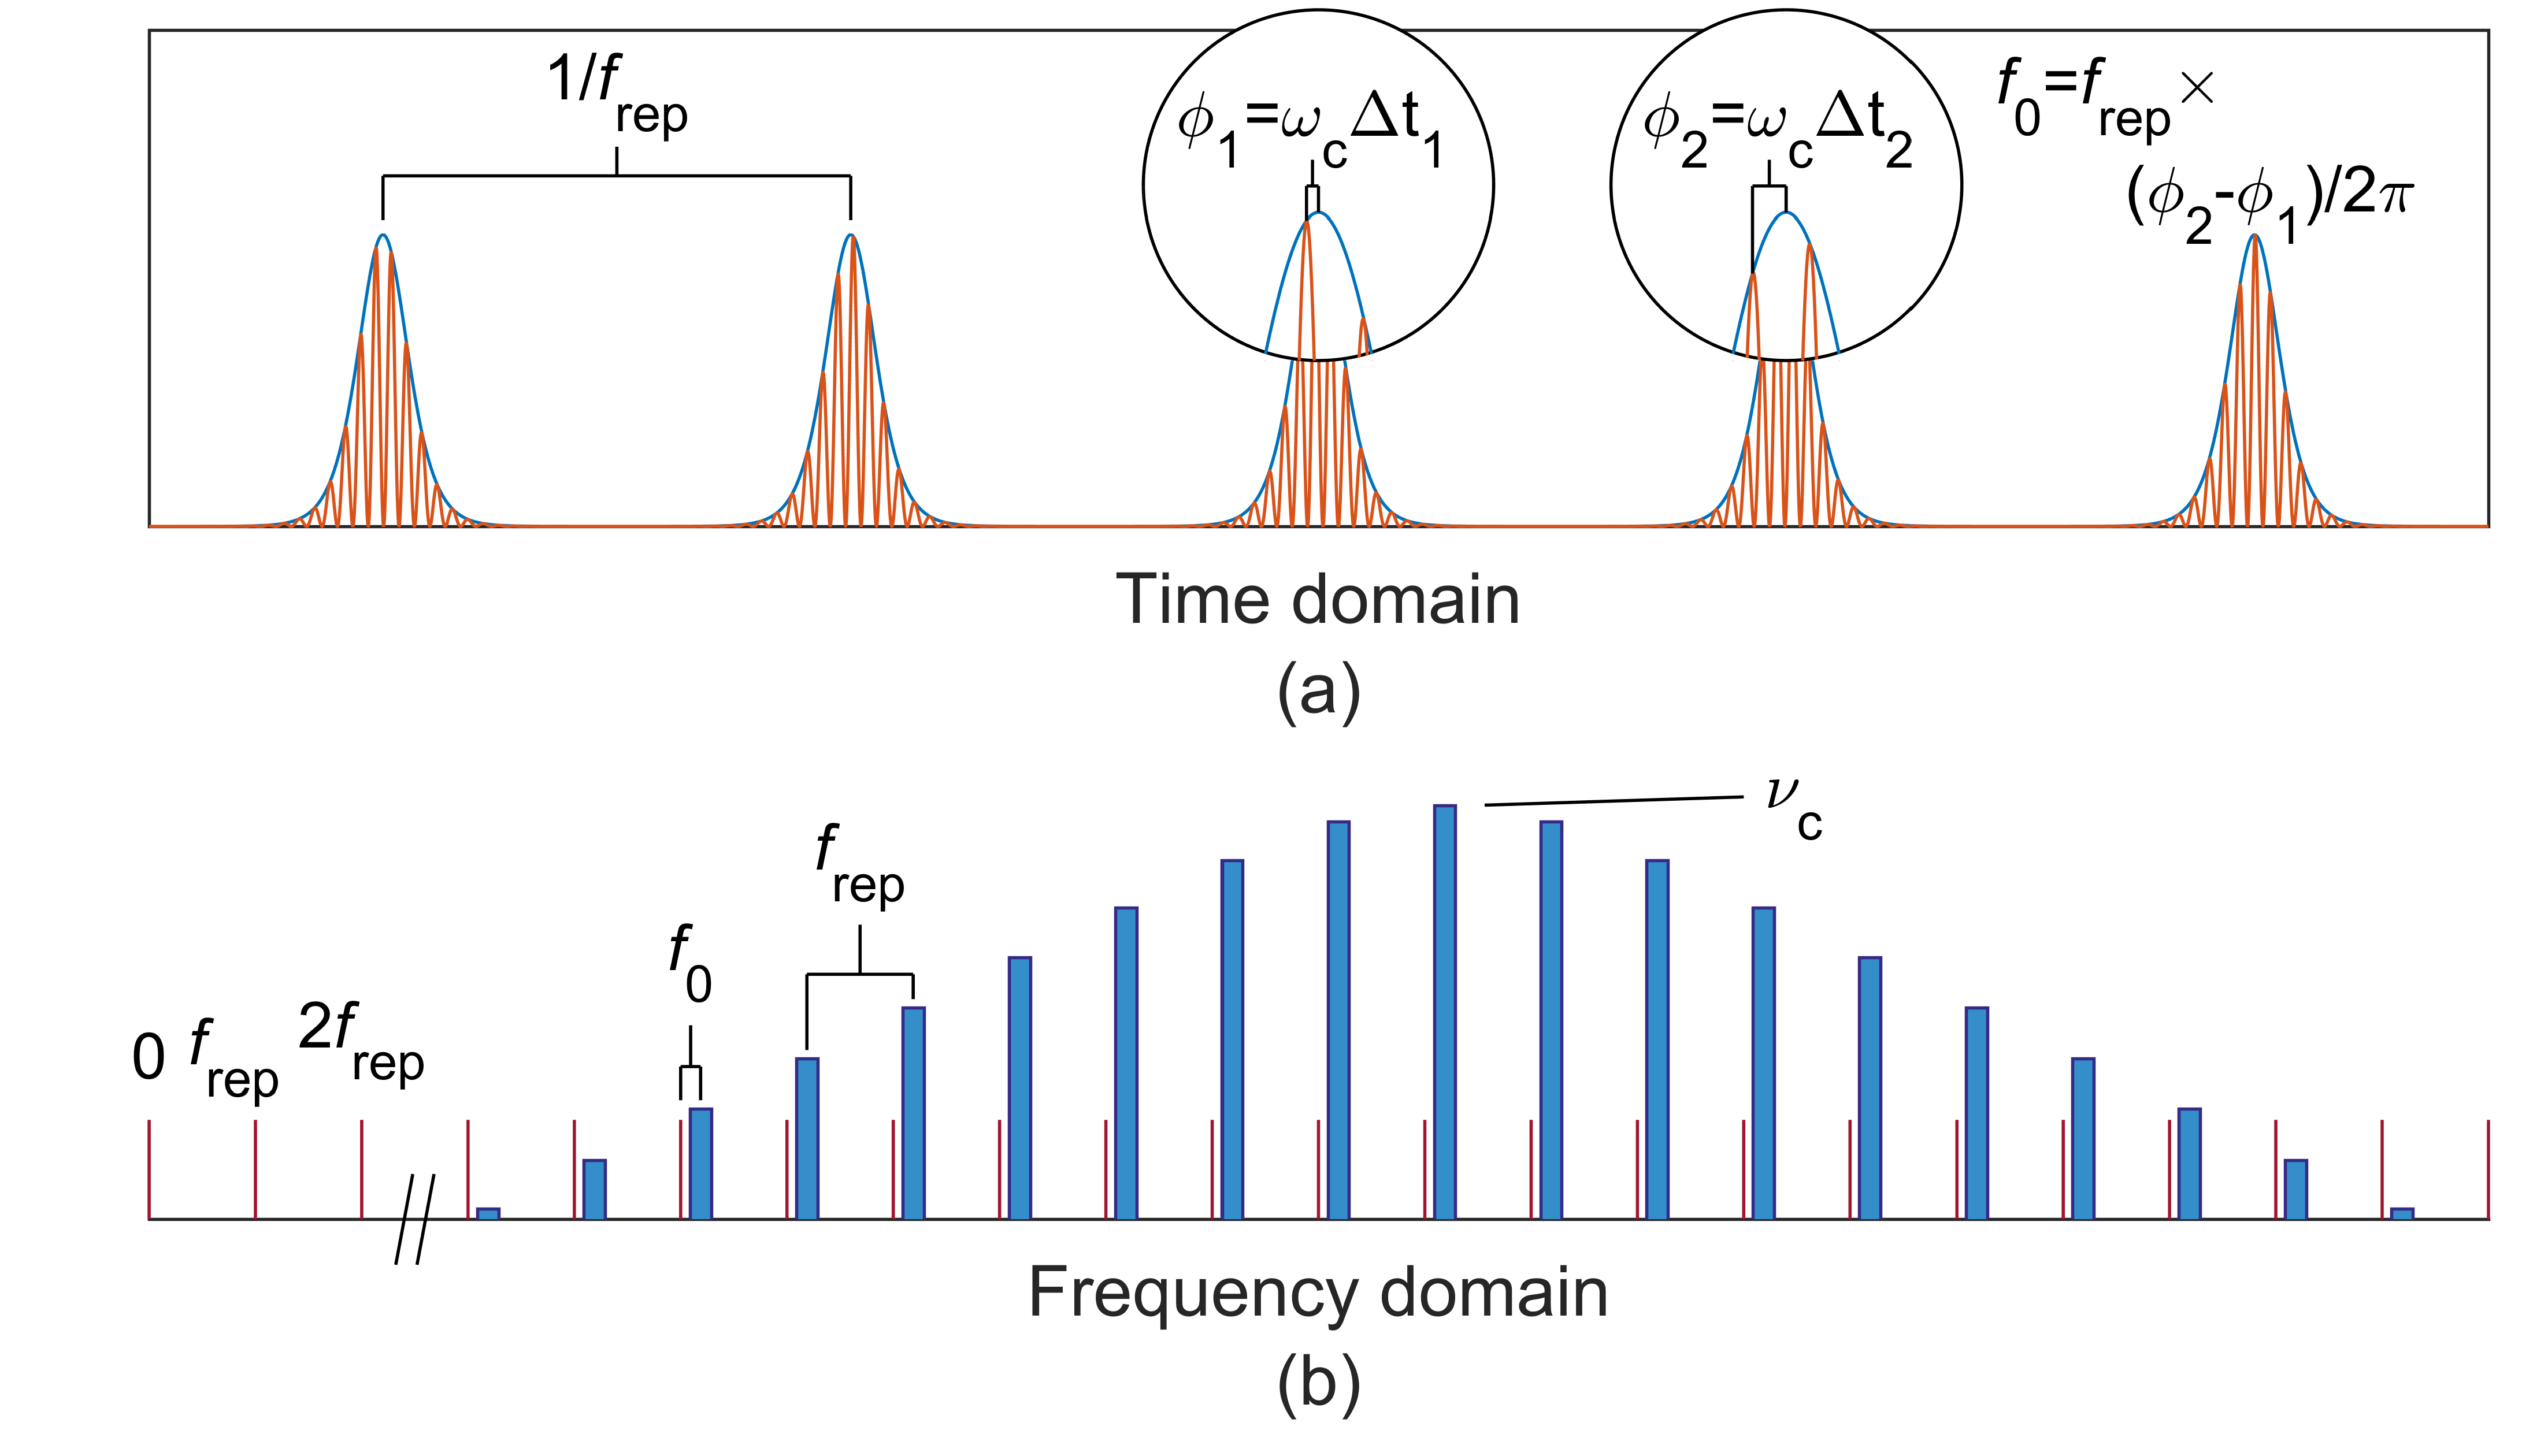
\includegraphics{\FigPath/Figures/Introduction/IntroFCbasics.png}
	\end{center}
	\caption[Optical frequency combs in the time and frequency domains]{\textbf{Optical frequency combs in the time and frequency domains.} (a) Time-domain depiction of a frequency comb as a train of pulses spaced by $1/f_{rep}$. The intensity envelope is shown in blue, and the carrier wave is shown in orange. The carrier-envelope offset frequency $f_0$ arises from a phase-slip of the carrier with respect to the intensity envelope from pulse to pulse. Specifically, if phases $\phi_j=\omega_c\Delta t_j$ are traced out by the carrier wave between its maximum and the $j$\textsuperscript{th} peak of the pulse train, then $f_0=\frac{\phi_{j+1}-\phi_j}{2\pi}f_{rep}$. (b) Frequency-domain depiction of the same frequency comb. The comb modes (shown in blue) are centered around an optical frequency $\nu_c$ and offset from harmonics of the repetition rate $f_{rep}$ (shown in red) by a frequency shift $f_0$. Note that the x-axis has been broken, and the zero-referenced mode numbers of the comb modes shown are large, e.g. $n\sim19340$ for a 10 GHz repetition-rate comb centered at 1550 nm wavelength (see Chapter \ref{chap:EOMCombs}). }
	\label{fig:CombBasics}
\end{figure} 



It is useful to consider a mathematical treatment of an optical pulse train to understand the relationships presented above. In the time domain, the electric field $E(t)$ of the pulse train consists of optical pulses that arrive periodically and have baseband (centered at zero frequency) field envelope $A(t)$ multiplying the carrier wave of angular frequency $\omega_c=2\pi\nu_c$:
\begin{equation}
E(t)=\sum_{k=-\infty}^{\infty} A(t-kT)e^{i\omega_c t}. \label{eq:pulsetrain}
\end{equation}
Here, $T$ is the repetition period of the pulse train. Eq. \ref{eq:pulsetrain} can be viewed as describing a laser of angular frequency $\omega_c$ with a time-varying amplitude. This temporal modulation leads to the distribution of the power across a spectrum whose width scales inversely with the temporal duration of $A$. Intuitively, the spectrum of the comb is the spectrum of the periodic baseband field envelope\footnote{which, as the spectrum of a periodic function, is already a comb.} $\Sigma_k A(t-kT)$, shifted in frequency by the multiplication with $e^{i\omega_c t}$ so that it is centered around the optical carrier. More formally, we can calculate the frequency content of the comb by calculating
\begin{equation}
\mathcal{F}\left\{E\right\}(\omega)\sim\left(\sum_{k=-\infty}^{\infty}\mathcal{F}\left\{A(t-kT)\right\}\right)*\delta(\omega-\omega_c).
\end{equation}
Here $\mathcal{F}$ denotes Fourier transformation and $*$ denotes convolution; this expression results from the Fourier transform's property that the transform of a product is the convolution of the transforms: $\mathcal{F}(A\cdot B)=\mathcal{F}(A)*\mathcal{F}(B)$. Now we use the Fourier transform's property that a temporal translation results in a linear spectral phase shift to obtain:
\begin{equation}
\mathcal{F}\left\{E\right\}\sim\left(\mathcal{F}\left\{A\right\}\times\sum_{k=-\infty}^{\infty}e^{-i\omega kT}\right)*\delta(\omega-\omega_c).
\end{equation}
The quantity $\Sigma_ke^{-i\omega kT}$ is the Fourier-series representation of the series of $\delta$-functions \mbox{$\Sigma_\mu\delta(\omega-2\pi\mu/T)$} (the \textit{Dirac comb}), so we have
\begin{equation}
\mathcal{F}\left\{E\right\}(\omega)\sim\left(\mathcal{F}\left\{A\right\}\times\sum_{\mu=-\infty}^{\infty}\delta\left(\omega-2\pi \mu/T\right)\right)*\delta(\omega-\omega_c),
\end{equation}
and performing the convolution leads to the replacement of $\omega$ with $\omega-\omega_c$, leading to:
\begin{equation}
\mathcal{F}\left\{E\right\}\sim\sum_{\mu=-\infty}^{\infty}\delta\left(\omega-\omega_c-\mu\omega_r\right)\mathcal{F}\left\{A\right\}(\omega-\omega_c), \label{eq:combspectrum}
\end{equation}
where $\omega_{rep}=2\pi f_{rep}=2\pi/T$. This expression indicates that the spectrum of the comb has frequency content at modes $\nu_\mu=\nu_c+\mu f_{rep}$, and that their amplitudes are determined by the spectrum of the baseband field envelope, shifted up to the optical carrier frequency $\nu_c$. This is the natural formulation in the case of a comb derived from a CW laser, but it obscures the carrier-envelope offset frequency in the difference between $\nu_c$ and the nearest multiple of the repetition rate, as discussed above. In practice, if $f_{rep}$ is known, then a measurement of $f_0$ is equivalent to a measurement of the frequency of the input CW laser.


\subsection{Frequency stabilization of optical pulse trains}

The scientific need for a method to measure optical frequencies motivated the development of optical frequency combs. While the measurement bandwidth of electronic frequency counters has improved since 1999, it remains limited to frequencies roughly \textit{ten thousand} times lower than the frequency of, e.g., visible red light. Frequency combs present a method for measurement of the unknown frequency $f_{opt}$ of an optical signal through heterodyne with a frequency comb---if $f_{opt}$ falls within the bandwidth of the frequency comb, then the frequency of the heterodyne between the comb and the signal is guaranteed to be less than $f_{rep}/2$. If the frequencies of the comb are known, measurement of the heterodyne with the signal reveals its frequency  $f_{opt}$, provided that the comb mode number and sign of the beat can be determined. This can be done via a wavelength measurement if sufficient precision is available, or by measuring the change $\partial f_b/\partial f_{rep}$, where $f_b$ is the measured frequency of the beat.

The utility of the optical frequency comb lies in the fact that measurement of the two frequencies $f_{rep}$ and $f_0$ is sufficient to determine the optical frequencies of all of the modes of the comb, thereby enabling frequency measurement of optical signals. Measurement of the repetition rates of optical pulse trains was possible before the realization of optical frequency comb technology, as this can be done by simply impinging the pulse train on a photodetector. Some pulse trains generated in new platforms have repetition rates too high for direct measurement in this way, but this challenge can be addressed by e.g. spectrally interleaving a lower repetition-rate comb \cite{Spencer2018,Briles2017}. In general, measurement of $f_0$ presents the more difficult challenge. It was the confluence of several technological developments around the turn of the twenty-first century that allowed detection and measurement of this frequency, thereby enabling creation of fully-stabilized modelocked-laser pulse trains: optical frequency combs.

The carrier-envelope offset frequency of a pulse train is challenging to measure because it describes evolution of the optical carrier wave underneath the intensity envelope, and therefore cannot be measured through straightforward detection of the intensity of the pulse train. Presently, the most straightforward way to measure $f_0$ is $f-2f$ \textit{self-referencing}. This can be performed only with a pulse train whose spectrum spans an octave---a factor of two in frequency. Given such an octave-spanning supercontinuum spectrum, a group of modes near mode number $N$ is frequency-doubled in a medium with the $\chi^{(2)}$ nonlinearity \cite{Boyd2003}. This frequency-doubled light is heterodyned with the native light in the supercontinuum with mode number near $2N$. The frequency of the resulting beat $f_b$ is:
\begin{align}
f_b&=f_{doubled}-f_{native}\\
&=2(Nf_{rep}+f_0)-(2Nf_{rep}+f_0)\\
&=f_0.
\end{align}
Such a scheme is implemented in an $f-2f$ \textit{interferometer}, which is depicted in Fig. \ref{fig:f2f}. Generating the necessary octave-spanning supercontinuum spectrum typically requires nonlinear spectral broadening of the pulse train after its initial generation except for in specific, carefully engineered cases (e.g. \cite{Briles2017,Fortier2003}). Achieving the required degree of spectral broadening while preserving the coherence properties of the pulse train is a significant challenge---in the past this has typically required launching a train of high energy ($\sim$1 nJ), temporally short ($\leq$ 100 fs) pulses into the spectral-broadening stage. Recent developments in nonlinear fiber and waveguide technology have relaxed these requirements slightly (e.g. Ref. \cite{Carlson2017}, also Chapter \ref{chap:EOMCombs}), but maintaining the coherence of the pulse train during spectral broadening remains an important consideration in designing optical frequency comb systems. 

The application of $f-2f$ self-referencing for full frequency-comb stabilization is discussed in Chapters \ref{chap:EOMCombs} and \ref{chap:PulsePicking}. Self-referencing of microresonator-based frequency combs is not a result presented explicitly in this thesis, but it is nonetheless a key step in the preparation of microcombs for applications and is a  motivation for the investigations into microcomb nonlinear dynamics that are presented in Chapters \ref{chap:PMPumping}-\ref{chap:FPLLE}.


\begin{figure}[htpb]
	\begin{center}
		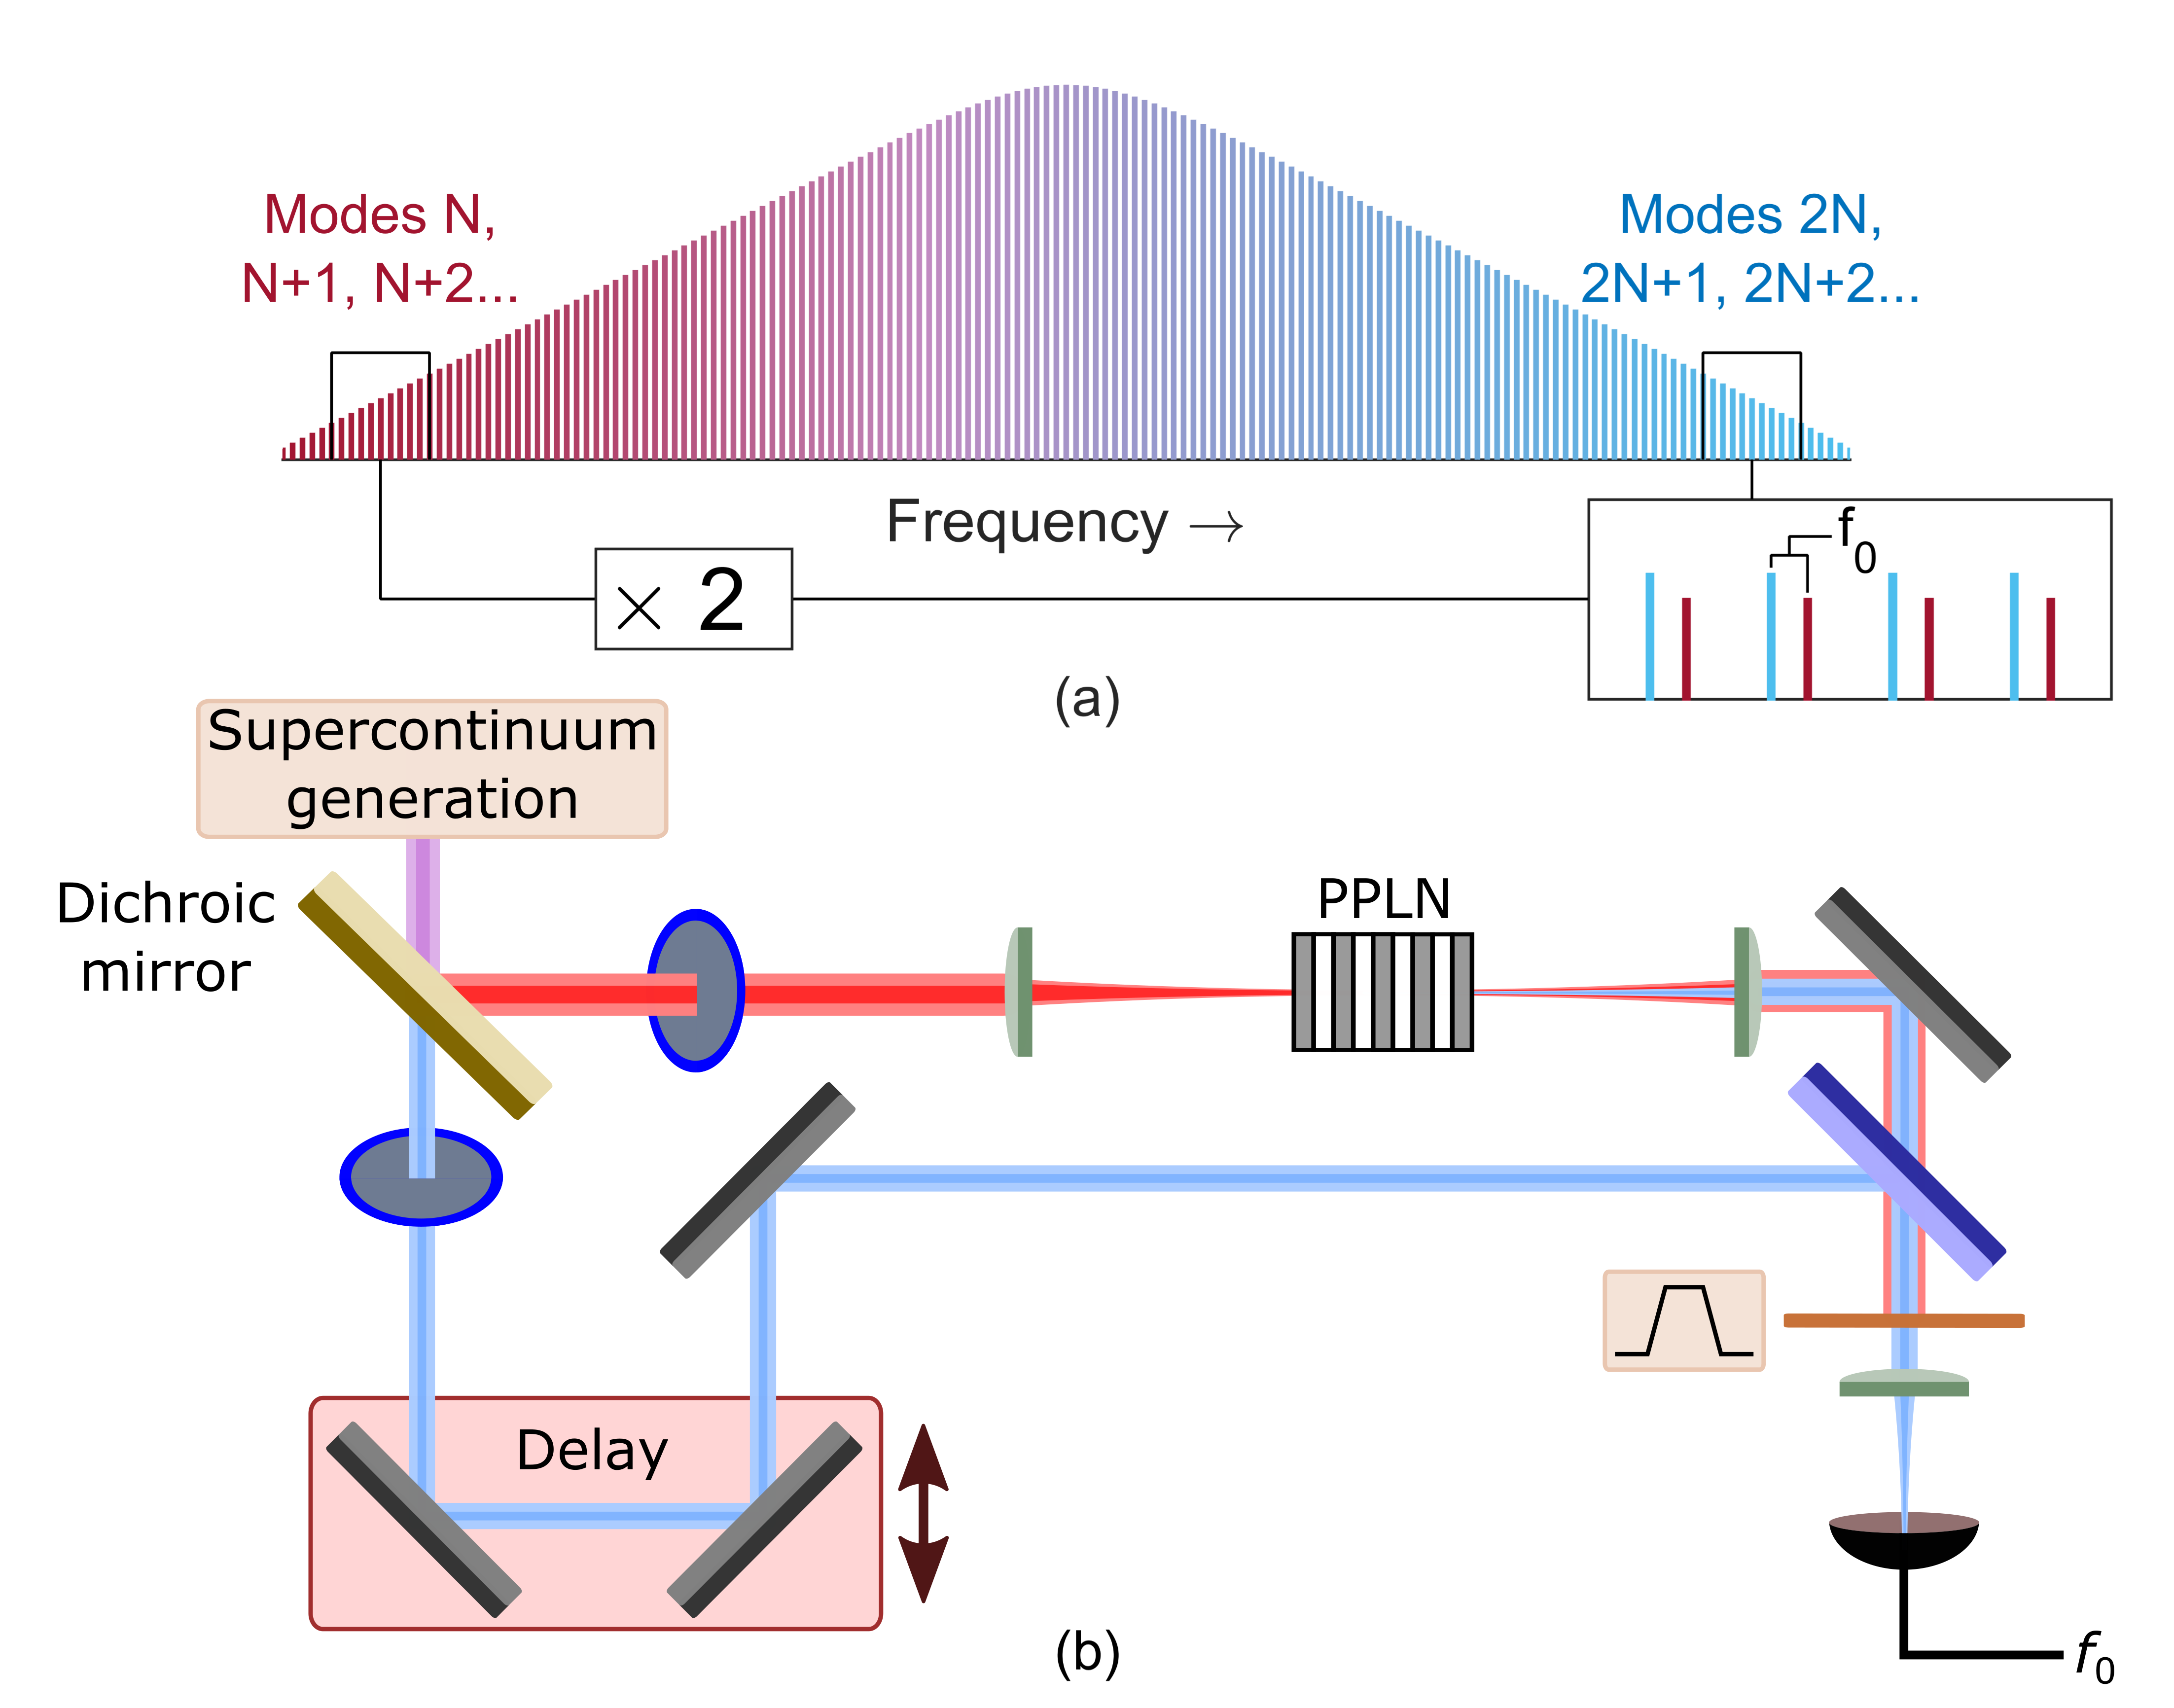
\includegraphics{\FigPath/Figures/Introduction/Introf2fv4.png}
	\end{center}
	\caption[Measurement of the carrier-envelope offset frequency via $f-2f$ self-referencing]{\textbf{Measurement of the carrier-envelope offset frequency $f_0$ via $f-2f$ self-referencing.} (a) Frequency-domain depiction of $f-2f$ self-referencing: Light on the low frequency end of an octave-spanning supercontinuum is frequency-doubled, and then heterodyned with light on the high frequency end near twice its frequency, enabling measurement of the carrier-envelope offset frequency. (b) Schematic depiction of an $f-2f$ interferometer: After supercontinuum generation, a dichroic mirror splits the light by wavelength, and the low-frequency end of the supercontinuum (red) is sent through a nonlinear crystal for frequency-doubling. Here the crystal is periodically-poled lithium niobate (PPLN), where quasi-phasematching is employed for efficient doubling of the target modes \cite{Hum2007}. The high-frequency end (blue) is sent through a delay stage, which can be adjusted to compensate for temporal walk-off between the spectral components (modes $\sim N$ and modes $\sim 2N$) required for self-referencing during the supercontinuum generation process. The two beams are then recombined by a beamsplitter and sent through a narrow optical band-pass filter centered around the doubled modes, which filters out light not necessary for $f_0$ measurement to increase the signal-to-noise ratio of the detection. Photodetection of the band-passed beam then reveals $f_0$. Waveplates in each path are used to optimize the polarization of the long-wavelength light for frequency-doubling and to ensure co-polarization of the two beams on the detector. }
	\label{fig:f2f}
\end{figure} 
 %Introduction
%\include{Experiment}
%\include{ATI} 
% \chapter{EOM Combs}

In this chapter, I discuss the generation of high-repetition-rate frequency combs through electro-optic modulation of a continuous-wave laser – so-called EOM combs \cite{Kobayashi1972,Kourogi1993,Murata2000,Sakamoto2007,Morohashi2008,Ishizawa2010,Wu2010,Supradeepa2012,Metcalf2013,Wu2013}. This scheme represents an alternative to parametric generation of HRR combs in Kerr resonators, and as the technology matures it will likely find a niche in the application space that leverages its long-term stability, lack of moving parts, and possibility for robust turn-key operation. First I present the operational principle, and then experimental results that represent the first generation of a coherent octave-spanning supercontinuum and detection of an active-modulation-based frequency comb's carrier-envelope offset frequency without an external optical reference. Then I provide a detailed discussion of the noise properties of the EOM comb, the investigation of which is a significant contribution of the work described here. Finally, I provide a discussion of some possible future directions for the technology.

\section{Principle of operation}
Generally, the EOM comb concept consists of passing a CW 'seed' laser through cascaded phase and intensity modulators to generate a train of chirped pulses, and then propagating this pulse train through a dispersive medium to temporally compress the pulses to near their bandwidth-limited pulse duration. An generic expression for the electric field before temporal compression results from the product of the field $E_oe^{-i\omega_ct}$ with operators
\begin{align} \frac{1}{2}\left\{\mathrm{exp}\left[i(\phi_{DC}+\phi_{RF}\sin{\omega_rt})\right]+\mathrm{exp}\left[-i(\phi_{DC}+\phi_{RF}\sin{\omega_rt})\right]\right\}\\
=\cos\left(\phi_{DC}+\phi_{RF} \sin(\omega_rt+\phi_{IM-PM})\right)
\end{align} representing the intensity modulation and 
\begin{equation}
\mathrm{exp}\left[i\beta_m \sin{\omega_r t}\right]
\end{equation} representing the phase modulation. Here $E_o$ and $\omega_c$ are the complex amplitude and the carrier frequency of the seed laser. The phases  $\phi_{DC}$ and $\phi_{RF}$ represent the DC bias and depth of the intensity modulation, respectively, which experimentally are sourced from a DC power supply and an RF synthesizer. Writing the intensity-modulation operator as the sum of exponentials reveals the physical origin of intensity modulation as phase modulation in two paths with opposite sign. The phase-modulation index, which sets the initial bandwidth of the EOM comb, is $\beta_m$. The comb's repetition rate is $f_r=\omega_r/2\pi$, with $\omega_r$ the angular frequency of the phase and intensity modulation, which in practice are derived from the same synthesizer. The phase $\phi_{IM-PM}$ represents a phase difference between the IM and PM operators arising from path-length differences, which can be controlled via the insertion of a phase shifter in one electrical path. 

In practice, for subsequent spectral broadening of the comb it is desirable to configure the IM and PM to yield a train of 50 $\%$ duty-cycle pulses with normal chirp (temporally increasing carrier frequency). To achieve this, both $\phi_{DC}$ and $\phi_{RF}$ are set to $\pi/4$ and $\phi_{IM-PM}$ is set to zero. To achieve the former, the DC bias voltage and the RF modulation amplitude are adjusted to yield the appropriate optical spectrum for the seed laser with only intensity modulation applied. Setting $\phi_{IM-PM}$ to either zero or $\pi$ is achieved by examining the optical spectrum of the EOM comb with both IM and PM applied. The spectrum is asymmetric if $\phi_{IM-PM}$ is not zero or $\pi$ due to stronger transmission of either the high- or low-frequency components of the phase-modulated seed laser through the intensity modulators. The optical spectrum of the comb, which does not include phase information, is the same for $\phi_{IM-PM}=0$ or $\pi$; the difference between the two corresponds to reversal of the field in time or, equivalently, the difference between normal and anomalous chirp. In practice, setting $\phi_{IM-PM}$ to zero can be achieved by verifying that the pulses are compressed by propagation in an appropriate length of an anomalously dispersive medium; $\phi_{IM-PM}=\pi$ corresponds to anomalous chirp.

A simplified and illuminating expression for the electric field of a normally-chirped 50 $\%$ duty-cycle pulse train (up to a constant overall phase shift relative to the previous expression) is:
\begin{equation}
E=E_o\cos\left(\frac{\pi}{2}\sin^2{\frac{\omega_rt}{2}}\right)e^{i\omega_ct-i\beta_m\cos{\omega_rt}}.
\end{equation}
This can be understood as the product of a time-varying real amplitude $a(t)=E_o\cos\left(\frac{\pi}{2}\sin^2{\frac{\omega_rt}{2}}\right)$ and a phase factor from which the instantaneous carrier frequency $\omega(t)=\omega_c+\omega_r\beta_m\sin{\omega_rt}$ can be calculated. The carrier frequency $\omega(t)$ is increasing when the amplitude $a(t)$ is at its maximum, corresponding to normal chirp on the pulses.


\section{Detection of the carrier-envelope offset frequency of an EOM comb}

Here I describe generation of an EOM comb with 10 GHz repetition rate and subsequent measurement of its carrier-envelope offset frequency. The experimental setup is depicted in Fig. 1a. The basic experimental scheme consists of the following steps: 1. Initial generation and temporal compression of the EOM comb pulse train; 2. Modest spectral broadening and temporal re-compression; 3. Noise reduction using a Fabry-Perot filter cavity; and 4. Octave-spanning supercontinuum generation and detection of the carrier-envelope offset frequency. The results described below represent the first time a frequency comb based on active modulation of a CW laser has been self-referenced. Key to the success of this approach is the implementation of nonlinear spectral broadening in two stages, which allows the second stage to be seeded with $\sim$130 fs pulses for coherent supercontinuum generation. The noise reduction stage is also critical for coherent spectral broadening, and the investigation of its effects is a significant contribution of this work. 

To generate the initial train of chirped pulses, a telecom-band continuous-wave laser is passed through cascaded phase and intensity modulators driven with a 10 GHz microwave signal. The intensity modulator is biased at the 50 \% transmission point and driven with an RF amplitude appropriate for generation of a 50 $\%$ duty-cycle pulse train, as described above.   The phase modulator is driven with modulation depth of $\sim31\pi/4\sim24.3$ rad. The relative phase between the modulators is set such that the phase applied by the phase modulator is at a minimum when the transmission of the intensity modulator is highest; this yields a train of normally-chirped (up-chirped) pulses. Simulated temporal intensity and instantaneous carrier-frequency profiles are shown in Fig. 1b, and a simulated optical spectrum is overlaid on an experimental measurement in Fig. 1c.


\begin{figure}[htpb]
	\begin{center}
		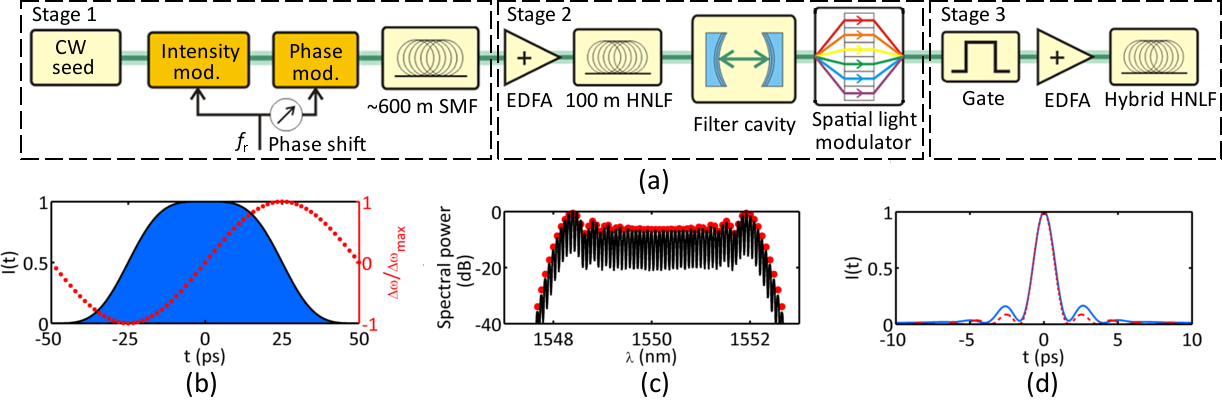
\includegraphics[width=15cm]{\FigPath/Figures/EOMCombs/EOMCSchematic.png}
	\end{center}
	\caption[Figure Title]{\textbf{Schematic and principle of operation for detection of the carrier-envelope offset frqeuency of an EOM comb.} (a) Experimental schematic for $f_0$ detection, with three stages: 1. Initial generation and temporal compression of the pulse train; 2. First stage of spectral broadening and temporal re-compression, along with noise suppression, and 3. Final stage of spectral broadening for generation of a coherent octave-spanning supercontinuum, including the implementation of an electro-optic gate for repetition-rate downsampling. (b) Depiction of a constituent pulse from a train of 50 $\%$ duty-cycle normally-chirped pulses with 10 GHz repetition rate. Intensity is shown in blue, and instantaneous carrier frequency is shown in red. The periodic electric field of this pulse train is given by Eqn. \ref{Eqn:EOMC} (c) Measured optical spectrum of the initial EOM comb pulse train (black), along with the simulated spectrum corresponding to the plots in panel (b). (c) Simulated temporal compression of the pulses shown in panel (b), with compression conducted by propagation in 570 m of SMF (solid blue) and compression to the transform limit (dashed red). The full-width at half-maximum (FWHM) duration of both pulses is $\sim$1.5 ps.   }
	\label{fig:EOMC_Schematic}
\end{figure} 


Next, the chirped pulse train is propagated through 600 m of anomalously-dispersive SMF. The length of SMF that is appropriate for pulse compression depends on the bandwidth of the optical pulses to be compressed; equivalently, it depends on both the phase-modulation depth and the repetition rate of the pulse train. This temporal compression reduces the duration of the optical pulses from $\sim$50 ps to $\sim$ 1.5 ps. A simulation of the resulting intensity profile is presented in Fig. 1d. 

The compressed pulses are amplified to 400 mW average power in an erbium-doped fiber amplifier and launched into 100 m of HNLF. This section of HNLF has chromatic dispersion that is small and normal; this is carefully chosen to chirp the pulses via self-phase modulation while avoiding soliton-fission dynamics\cite{Dudley2006}. The result is a train of chirped $\sim$1.5 ps pulses exiting the fiber.  In Fig. 2a we present the measured optical spectrum of this pulse train, as well as results of a numerical simulation of the spectral broadening in the 100 m of normally-dispersive HNLF. These simulations are conducted using the nonlinear Schrodinger equation (NLSE) including third order dispersion\cite{Agrawal2007}, taking as initial conditions the calculated intensity profile of the EOM comb pulses shown in Fig. 1d. The dispersion values for the HNLF used in the simulation are $D=-0.04$  ps/nm$\cdot$km and $D'=0.003$ ps/nm$^2\cdot$km, close to the values specified by the manufacturer. The simulation method is described in detail in App. \ref{NumericalSims}.

After propagation through the first section of HNLF, the pulses are passed through a high-finesse Fabry-Perot cavity for suppression of optical frequency fluctuations as discussed below. Then the pulses are temporally compressed again, this time using a commercial spatial light modulator (SLM) \cite{Weiner2000}; the SLM separates narrow spectral regions using a grating and passes them through individually controlled delaying elements before recombination. The SLM applies 2\textsuperscript{nd}, 3\textsuperscript{rd}, and 4\textsuperscript{th} order chromatic dispersion, which simulations indicate is sufficient to compress the chirped pulses to $\sim$130 fs, near their transform limit. This is shown in Fig. 2b. While it is convenient, the SLM is not strictly necessary; it would also be possible to compress the pulses via propagation in an appropriate length of SMF. Figs. 2b and 2c present the output intensity profile and the evolution of the intensity profile, respectively, in simulated compression in SMF. Because the pulses are broadband, temporally short, and reasonably high energy, these simulations include the full dispersion profile of SMF and the Kerr nonlinearity.



The temporally compressed $\sim$130 fs pulses are then passed through a Mach-Zehnder modulator functioning as an electro-optic gate for repetition-rate downsampling (see Chapter \ref{PulsePicking}). The gate selectively transmits every fourth pulse, reducing the repetition rate of the pulse train to 2.5 GHz. This facilitates coherent supercontinuum generation in a second stage of spectral broadening by increasing the pulse energy that can be achieved at a given average power. Note that this step is convenient but not strictly necessary, as shown in Ref. \cite{Beha2017}. 

The downsampled 2.5 GHz pulse train is amplified to an average power of 1.4 W, resulting in a train of $\sim$0.56 nJ pulses. This pulse train is propagated through 8 m of hybrid HNLF, yielding the spectrum shown in Fig. 2d. This hybrid HNLF consists of two segments with different dispersion profiles, with each segment serving a different purpose. The first segment is 30 cm long and highly dispersive ($D=6$  ps/nm$\cdot$km), and generates a dispersive wave centered at 1090 nm. The second segment is 7.7 m long and has lower dispersion ($D=1.5$  ps/nm$\cdot$km), and generates a Raman-self-frequency-shifted soliton centered near 2150 nm. The effect of each of these fibers on the output spectrum can be understood by investigating propagation in each section separately. To do this we use the LaserFOAM program \cite{Amorim2009}, which employs the generalized NLSE including Raman scattering, self-steepening, and 2nd- through 4th-order dispersion. The simulations are run independently, and both take as their initial conditions 170 fs Gaussian pulses with 350 pJ energy, close to the energy coupled into the HNLF after accounting for losses. The results of these simulations are plotted in Fig. 2d. 

 % % % % % PulsePickedTrains]
\begin{figure}[htpb]
	\begin{center}
		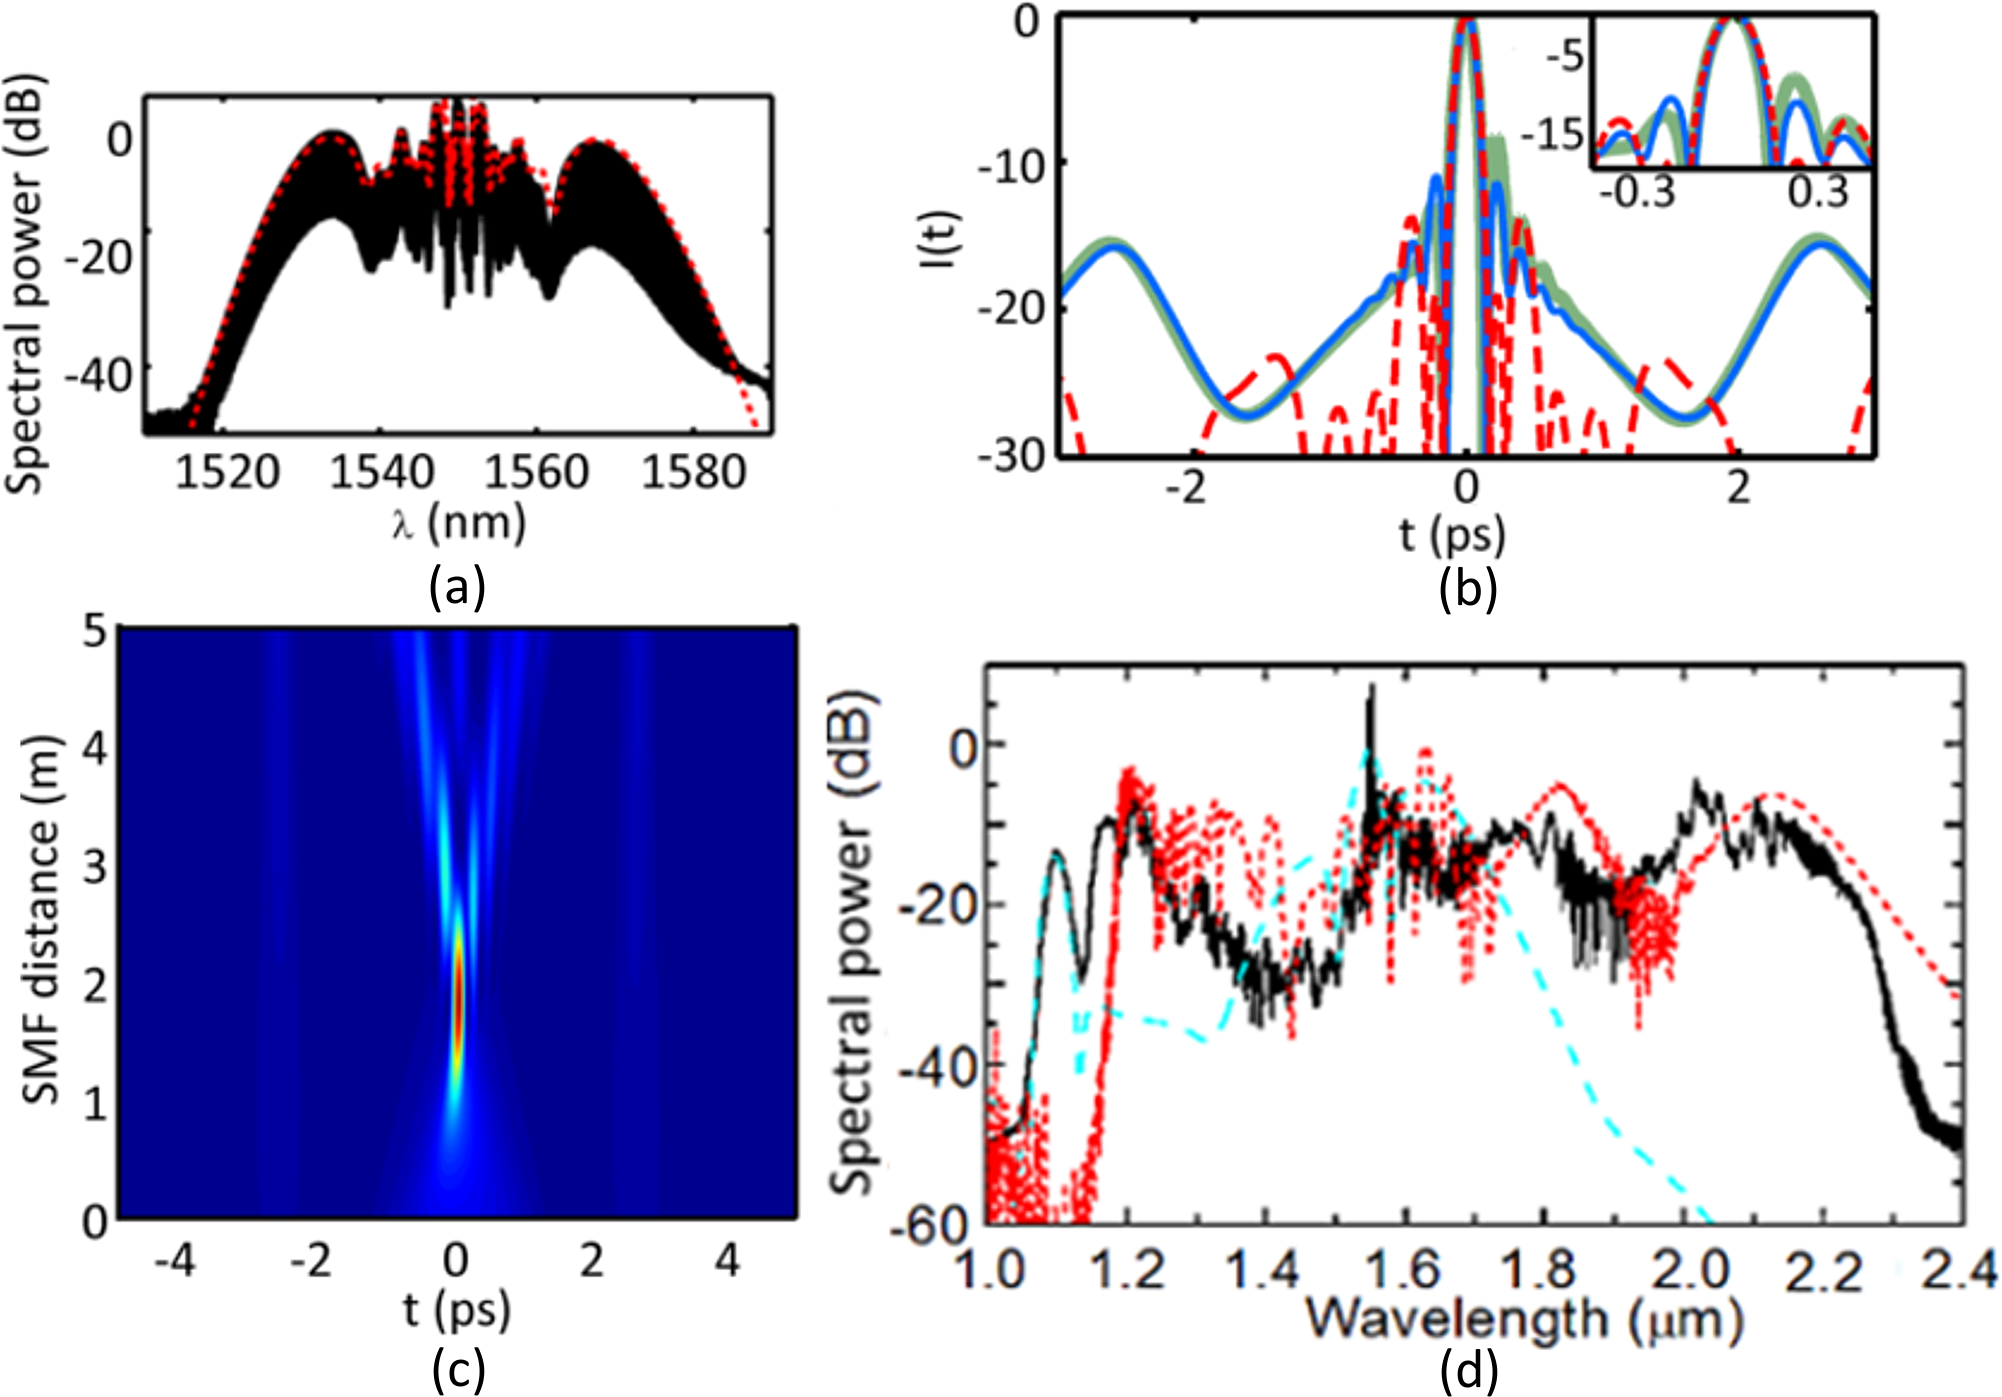
\includegraphics{\FigPath/Figures/EOMCombs/EOMC_spectraWsims.png}
	\end{center}
	\caption[Figure Title]{\textbf{Spectral broadening for generation of an octave-spanning supercontinuum.} (a) Measured optical spectrum after propagation in 100 m of low-normal-dispersion HNLF (black). The spectrum is broadened by self-phase modulation, which imposes a chirp on the pulses. Shown in red is a simulation of the same, conducted as described in the text. (b) Logarithmic-scale plot of the simulated pulse intensity envelopes after temporal recompression in the SLM with 2\textsuperscript{nd}-, 3\textsuperscript{rd}-, and 4\textsuperscript{th}-order dispersion (blue), in an appropriate length of SMF (thick green), to the transform limit (dashed red). (c) Simulated re-compression of the SPM-chirped pulses (red spectrum in panel (a)) in SMF. (d) Measured optical spectrum of the octave-spanning supercontinuum generated by the EOM comb system (black), plotted along with simulated spectra calculated as described in the text to investigate the effects of the 30 cm, highly-dispersive piece of HNLF (long-dashed teal) and the 7.7 m, lower-dispersion piece of HNLF (short-dashed red).}
	\label{fig:EOMC_Broadening}
\end{figure} 

The supercontinuum generated in the hybrid HNLF is coherent and suitable for $f-2f$ self-referencing (see App. \ref{App:f-2f}). To detect the carrier-envelope offset frequency of the EOM comb, we pass the pulse train through an interferometer consisting of a dichroic mirror, a delay stage in one path, and a 10 mm sample of periodically-poled lithium niobate that generates the second harmonic of supercontinuum light at 2140 nm.  The dichroic mirror and delay stage enable adjustment of the relative timing between the native 1070 nm and doubled 2140 nm components of the supercontinuum so that they are temporally coincident. An optical band-pass filter centered at 1070 nm selects the supercontinuum components required for self-referencing, shown in Fig. 3a, and impinging the filtered light on a photodetector reveals the carrier-envelope offset frequency of the EOM comb, shown in Fig. 3b. Note that downsampling introduces an ambiguity in the offset frequency due to the increased density of comb modes in the downsampled pulse train; this ambiguity can be removed by measuring the change in measured offset frequency with a change in $f_r=\omega_r/2\pi$ provided by the synthesizer driving the modulators. 




\begin{figure}[htpb]
	\begin{center}
		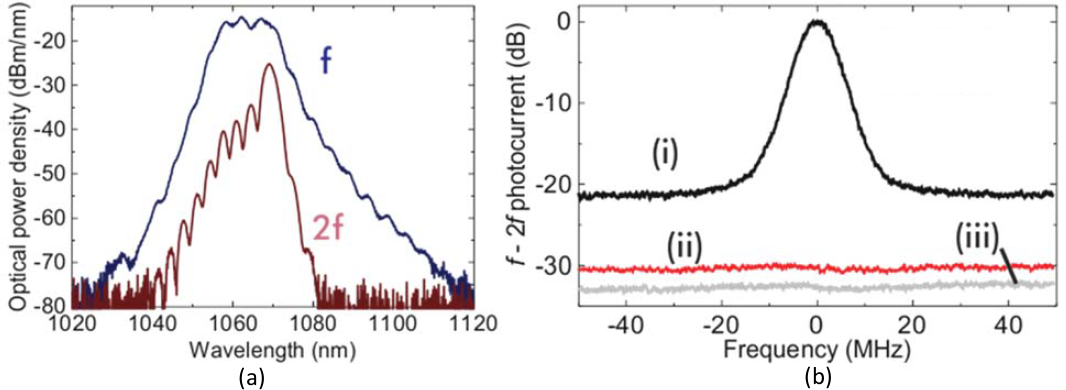
\includegraphics[width=15cm]{\FigPath/Figures/EOMCombs/EOMC_f0fromOptica.png}
	\end{center}
	\caption[Figure Title]{\textbf{Self-referencing of an EOM comb.} (a) Spectral components used for $f-2f$ self-referencing after passing through a 1070-nm optical bandpass filter: \color{red}native supercontinuum light (blue) and frequency-doubled 2140-nm supercontinuum light (red) ARE THESE LABELED CORRECTLY\color{black}. (b) Photodetected carrier-envelope offset frequency signal (black), along with a measurement of the intensity noise of the pulse train obtained by \color{red} blocking one of the paths (red) \color{black}and the photodetector noise floor (grey). \color{red}The intensity-noise measurement highlights the presence of a broad background noise floor  on the $f_0$ signal that must be the result of frequency fluctuations because it is not present when photodetecting either path alone.\color{black}}
	\label{fig:EOMC_f0}
\end{figure} 



\section{Noise in EOM Combs}

An important difference between the EOM comb scheme and other approaches for generation of frequency combs is that the repetition rate is derived from a microwave source and is multiplied directly by a factor $N$ to yield the optical frequency of the frequency-comb mode with number $N$ referenced to the seed laser (where $N=0$). Therefore, the contribution to the optical frequency noise of mode number $N$ from the microwave source scales with the mode number $N$, and the contribution to the power spectrum of frequency noise scales as $N^2$. This presents a challenge in the generation of coherent supercontinuum light, where the modes relevant for $f-2f$ self-referencing are far separated from the seed laser and $N$ is large. The factor by which the noise on the modulation tone $f_r$ is multiplied to determine its contribution to the noise on the measured carrier-envelope offset frequency is the ratio between the comb’s carrier frequency (the frequency of the seed laser) and the repetition rate: $N=f_c/f_r=$19340 for the 10 GHz comb discussed above (where $f_c=$193.4 THz for a 1550 nm seed laser). This contribution is shown in Fig. 3a, along with the contribution from the CW seed laser. The noise on $f_r$ results from technical noise on the synthesizer tone at low Fourier frequencies and approaches a white Johnson-Nyquist (thermal) phase-noise floor of -177 dBm/Hz at high Fourier frequencies. Noise in each of these regimes impacts the photodetected $f_0$ signal: low-frequency noise contributes to the linewidth of the comb modes and therefore the $f_0$ signal, while high-frequency noise contributes to a frequency-noise floor on the photodetected signal\cite{Domenico2010}. As discussed in Ref. \cite{Beha2017}, unmitigated multiplication of this noise floor by the factor $N^2=$19340$^2$ leads to a supercontinuum with optical frequency fluctuations that are large enough to prevent detection and measurement of $f_0$. 

To address this problem and enable $f-2f$ self-referencing of our comb, we pass the comb through a Fabry-Perot filter cavity whose free-spectral range is actively stabilized to the comb’s mode spacing. The filter cavity’s Lorentzian transfer function reduces the optical frequency fluctuations of the comb modes at high frequency – these fluctuations are averaged over the photon lifetime of the cavity. This enables generation of a supercontinuum with resolvable modes that is suitable for $f-2f$ self-referencing and measurement of $f_0$. 

The filter cavity used for this 10 GHz comb has a 7.5 MHz linewidth; equivalently, it has finesse of $F\sim$1333. The effect of passing the comb through the cavity is demonstrated concretely in Fig. 3b, where we compare the lineshape of a heterodyne beat between the supercontinuum and a CW laser with 1319 nm wavelength with and without the filter cavity in place. The signal-to-noise ratios for the beat with and without the filter cavity are 40 dB and 17 dB, respectively.


\begin{figure}[htpb]
	\begin{center}
		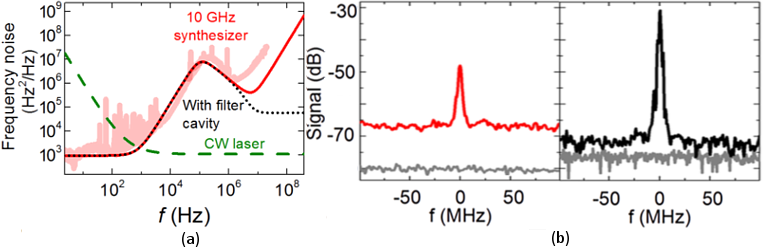
\includegraphics[width=15cm]{\FigPath/Figures/EOMCombs/EOMC_NoiseFigure_thesis.png}
	\end{center}
	\caption[Figure Title]{\textbf{Investigation of the noise properties of the EOM comb.}  (a) Contributions to the fluctuation spectrum of the carrier-envelope offset frequency: model of the input seed laser (dashed green), model of the 10 GHz synthesizer multipled by 19430$^2$ without the filter cavity (solid red, experimental data thick red), and synthesizer multiplied by 19340$^2$ and the Lorentzian filter-cavity transfer function (dotted black). (b) Comparison of the detected beats between the supercontinuum and a 1519 nm-wavelength CW laser without (red, left) and with (black, right) the Fabry-Perot filter cavity. The level of intensity noise on the supercontinuum, measured by removing the 1319 nm CW laser, is shown by the lower gray trace in each plot. Signal-to-noise ratios for the beat are 17 dB without and 40 dB with the filter cavity.}
	\label{fig:EOMC_noise}
\end{figure} 

We also explore the effect of low-frequency fluctuations in the modulation tone $f_r$ by changing the source of this tone. The $f_0$ signal shown in Fig. \ref{Fig:EOMC_f0}b is acquired with a tunable commercial synthesizer providing $f_r$. In Fig. \ref{Fig:EOMC_f0_sources} we show the detected $f_0$ signal with a dielectric-resonator oscillator and a sapphire oscillator providing $f_r$; these sources have less low-frequency noise, and the effect of this lower noise is readily apparent in the reduced linewidth of the $f_0$ signal.



\begin{figure}[htpb]
	\begin{center}
		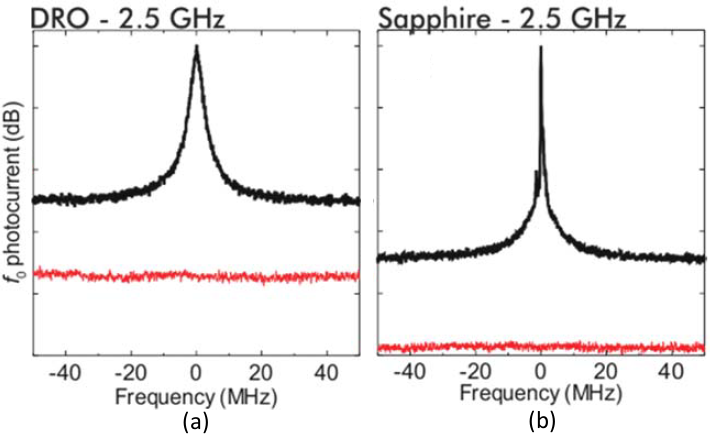
\includegraphics[width=10cm]{\FigPath/Figures/EOMCombs/EOMC_f0_diffosc_thesis.png}
	\end{center}
	\caption[Figure Title]{\textbf{Photodetected carrier-envelope-offset frequency signal with different sources for $f_r$.} (a) The $f_0$ beat resulting from a dieletric-resonator oscillator source for the modulation frequency. (b) Ibid with a sapphire oscillator as the source for $f_r$, which has lower noise than both the tunable commerical synthesizer and the DRO. The reduction in linewidth associated with the change in the source for $f_r$ shows the effect of low-Fourier-frequency noise of $f_r$ on the frequency-noise characteristics of the EOM comb. }
	\label{fig:EOMC_f0_sources}
\end{figure} 




% \chapter{Downsampling of optical pulse trains} \label{chap:PulsePicking}
    \begin{footnotesize}
 	\begin{spacing}{1.2}
 		This chapter describes work that was reported in:
 		\begin{itemize}
 			\item \fullcite{Cole2018b}.\\
 		\end{itemize}
 	\end{spacing}
 \end{footnotesize}
 

This chapter presents a discussion of a technique for repetition-rate reduction of optical pulse trains. While high pulse train repetition rates are appealing for some applications, they are not always appropriate. For example, spectral resolution in spectroscopy applications is sacrificed in a comb with a large mode spacing, and a high repetition rate makes nonlinear optics less efficient at a given average power. This can present a barrier to the generation of octave-spanning spectra for $f-2f$ self-referencing. On the other hand, in general the size of the comb package sets the scale for the round-trip time, meaning that low-SWAP combs tend to have inherently high repetition rates. Therefore, to increase the flexibility of low-SWAP and high repetition-rate comb systems in applications, a method for reducing the repetition rate of a pulse train will be useful.

We consider a method for pulse train repetition-rate reduction, or downsampling, in which an electro-optic gate realized by an RF-driven intensity modulator periodically transmits an incoming pulse at a frequency lower than the input repetition rate. The basic principle is illustrated in Fig. \ref{fig:PPConcept}. Downsampling via pulse gating, also referred to as `pulse picking' in the literature, has been used extensively in the context of high-field, phase-sensitive ultrafast optics for the generation of energetic, carrier-envelope-phase-stabilized ultrashort pulses \cite{Backus1998,Baltuska2003}. In this application, a comb with initial repetition rate in the $\sim$100 MHz range that has already been self-referenced and stabilized is pulse-picked to a repetition rate on the order of 1-100 kHz. Concerns in this application center around control and preservation of the carrier-envelope phase in the pulse-picking and amplification process \cite{Gohle2005,Rauschenberger2006}. In contrast, the focus here is on downsampling within the context of optical metrology with frequency combs, and we are concerned with downsampling's effect on the optical phase noise, the pulse-to-pulse energy fluctuations, and the carrier-envelope offset frequency of the comb. In particular, it is important that the downsampled pulse train is suitable for $f-2f$ self-referencing. 

Sec. \ref{sec:PPProofOfPrinciple} presents a proof-of-principle experiment in which a 250 MHz pulse train is downsampled to 25 MHz, and then spectrally broadened and self-referenced. A mathematical model of downsampling is presented in Sec. \ref{sec:PPMath}, and this model informs the discussion of downsampling's effect on the pulse train's noise properties presented in Sec. \ref{sec:PPNoiseExp} and Sec. \ref{sec:PPNoiseTheory}. In Sec. \ref{sec:PPAmplification} we discuss some practical considerations in applications of the technique, including the effect of imperfections in the gating process such as incomplete extinction of rejected pulses.



 % % % % % PulsePickedTrains]
\begin{figure}[htpb]
	\begin{center}
		%		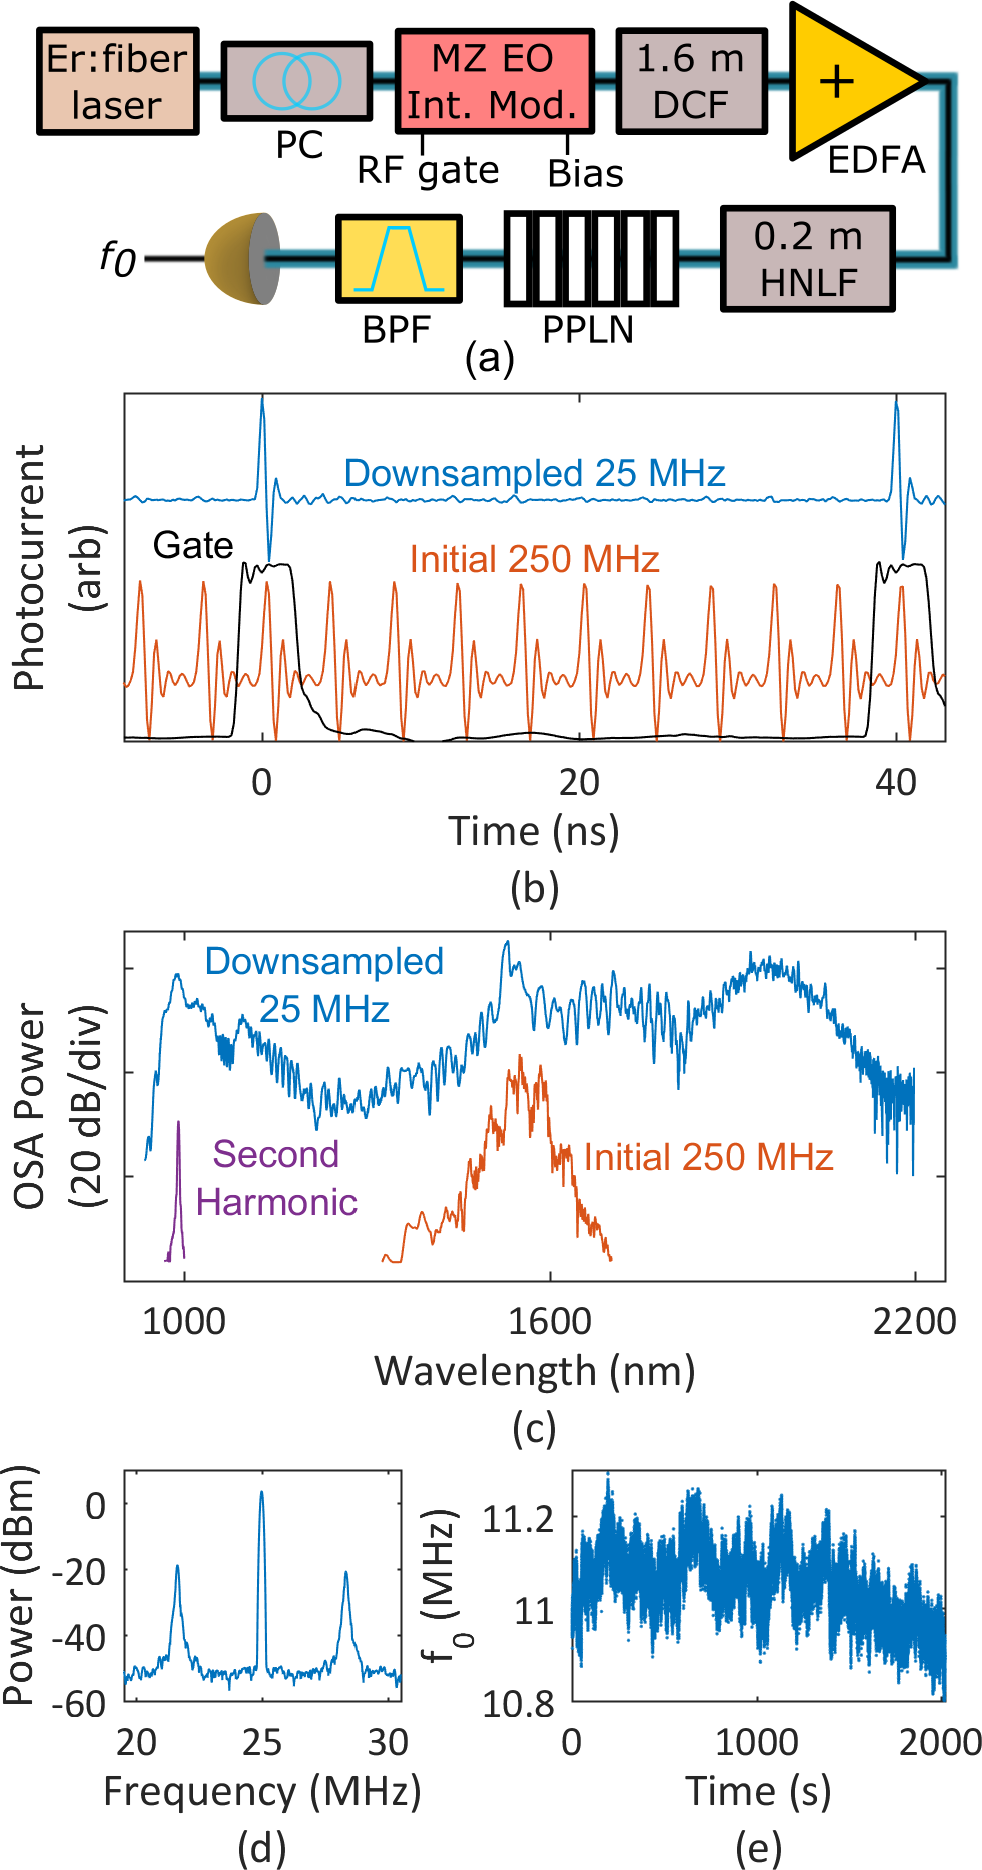
\includegraphics[width=110mm]{\FigPath/Figures/PulsePicking/PulsePickingPaperFig1.png}
		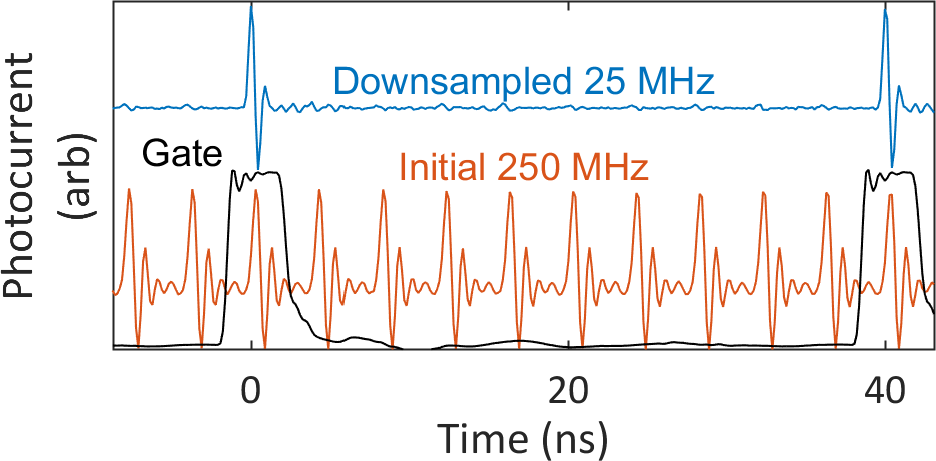
\includegraphics[width=110mm]{\FigPath/Figures/PulsePicking/PulsePickedTrains.png}
	\end{center}
	\caption[An illustration of pulse-train repetition-rate downsampling]{\textbf{An illustration of pulse-train repetition-rate downsampling.} Orange: A photodetected 250 MHz pulse train. Blue: A photodetected 25 MHz pulse train obtained by downsampling the 250 MHz pulse train by a factor of $N=10$. Black: Oscilloscope trace showing the voltage sent to the RF port of a Mach-Zehnder intensity modulator to selectively transmit a subset of the incoming pulses. With the intensity modulator biased for zero transmission, the voltage trace is indicative of the transmission.}
	\label{fig:PPConcept}
\end{figure} 





\section{Proof-of-Concept Experiment}\label{sec:PPProofOfPrinciple}
Here we present a proof-of-concept experiment in which a 250 MHz comb is downsampled and self-referenced. The setup for and results of this experiment are summarized in Fig. \ref{fig:PPDemo}. Our pulse gating scheme, shown in Fig. \ref{fig:PPDemo}a, employs a Mach-Zehnder (MZ) electro-optic intensity modulator driven by 25 MHz rectangular electronic gating pulses with 80 ps transitions and 3.5 ns duration. The electronic pulse generator and the repetition rate of the input 250 MHz comb are both referenced to a hydrogen maser to maintain synchronization. The DC bias of the intensity modulator is set for maximum extinction outside the electronic gate, whose amplitude is approximately matched to $V_\pi$ of the EOM. This downsampling scheme results in a stable 25 MHz optical pulse train with $>$12 dB contrast (Fig. \ref{fig:PPConcept}). This contrast is adequate for this experiment, but could be improved by cascading modulators with higher extinction ratios.  The average power of the 250 MHz pulse train is reduced from 30 mW to 400 $\mathrm{\mu}$W by the pulse gating process and the insertion loss of the optical components. The pulse train is amplified to 35 mW by use of a normal-dispersion erbium-doped fiber amplifier, which provides some spectral broadening and temporal pulse compression \cite{Fermann2000}. An octave-spanning supercontinuum is obtained by launching the amplified, $<$100 fs, $\sim$1 nJ pulses into 20 cm of highly nonlinear fiber (HNLF) \cite{Hirano2009}; the resulting spectrum is shown in Fig. \ref{fig:PPDemo}b.  For comparison, we also present the supercontinuum generated by the 250 MHz comb with the EOM set for constant maximum transmission under otherwise identical conditions. The 250 MHz comb is amplified by the same EDFA to an average power of 85 mW, corresponding to 340 pJ pulse energy, before it enters the HNLF.

To detect $f_0$, the octave-spanning supercontinuum shown in Fig. \ref{fig:PPDemo}b is sent into a free-space $f-2f$ interferometer consisting of a half-wave plate and a periodically poled lithium niobate (PPLN) crystal quasi-phasematched for second-harmonic generation at 1980 nm, as described in Sec. \ref{sec:f2f}. The generated 990 nm light is shown in \ref{fig:PPDemo}b. A 10 nm band-pass filter at 990 nm selects this second harmonic and the co-linear supercontinuum at 990 nm, which are then photodetected to observe $f_0$ with 30 dB signal-to-noise ratio, shown in Fig. \ref{fig:PPDemo}c. Fig. \ref{fig:PPDemo}d shows a 2000 s record of $f_0$ for the downsampled comb.




 % % % % % Bullet through Apple
\begin{figure}[htpb]
	\begin{center}
%		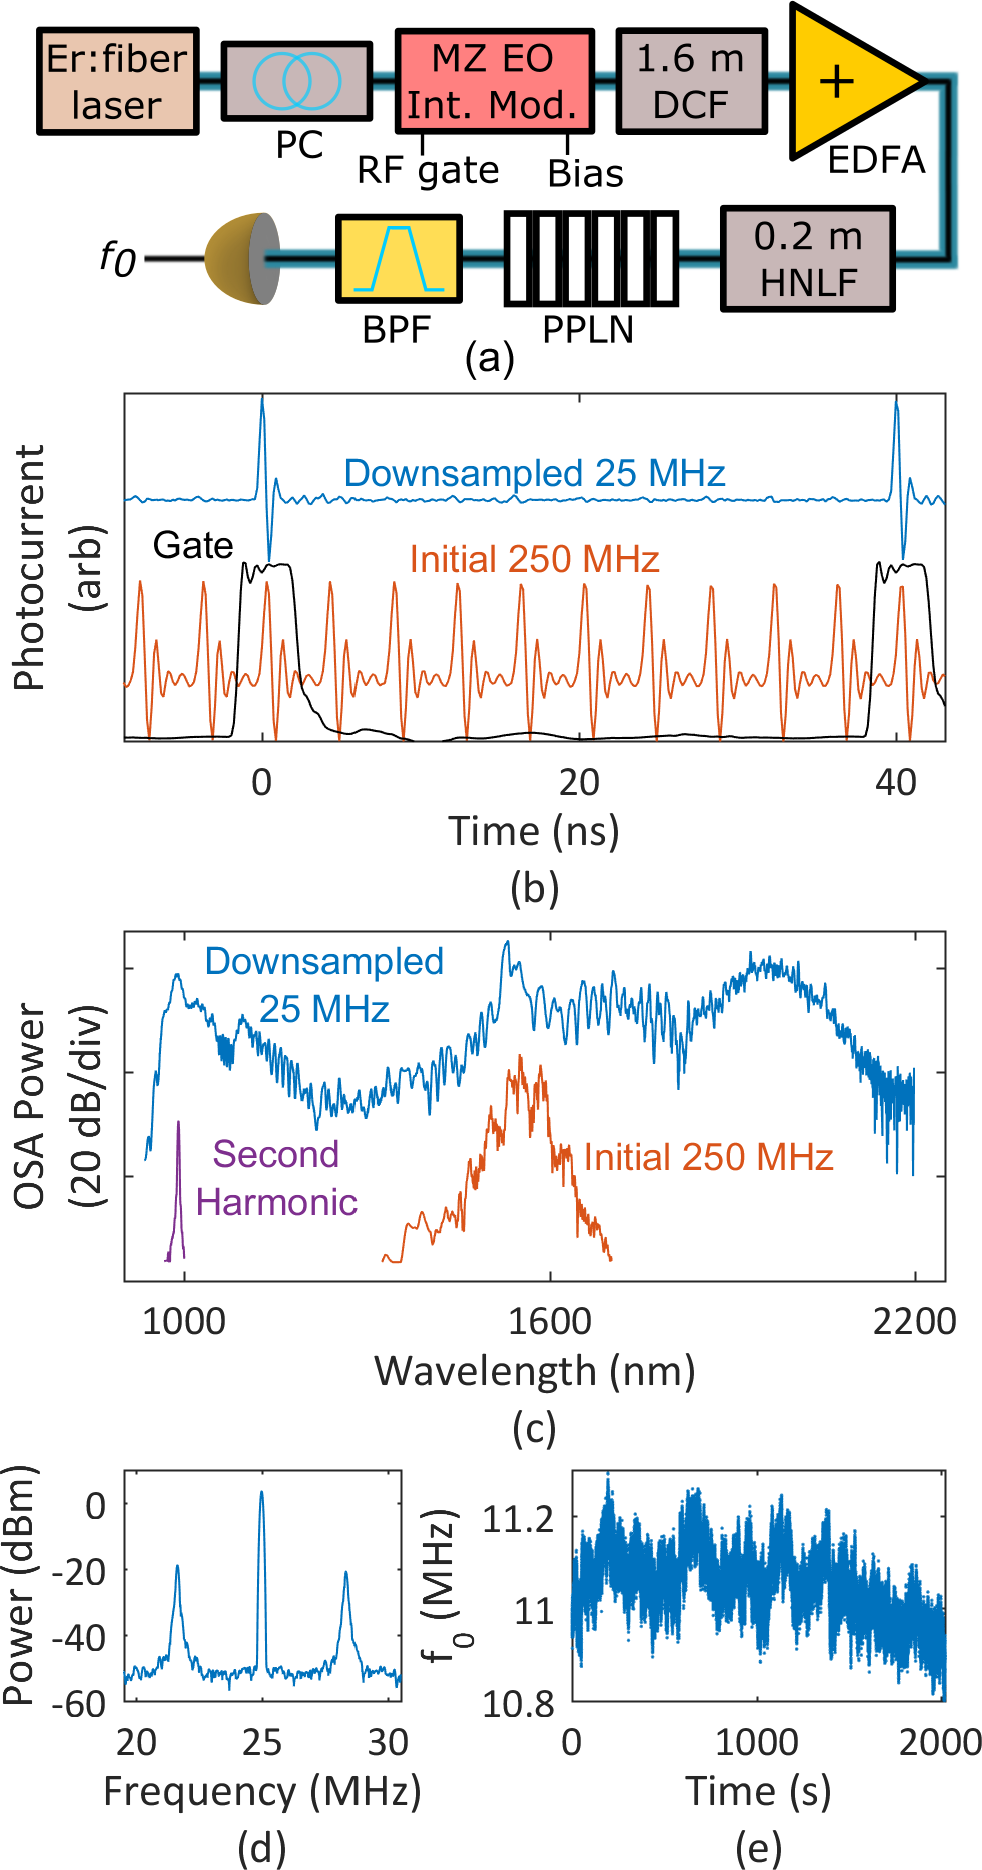
\includegraphics[width=110mm]{\FigPath/Figures/PulsePicking/PulsePickingPaperFig1.png}
		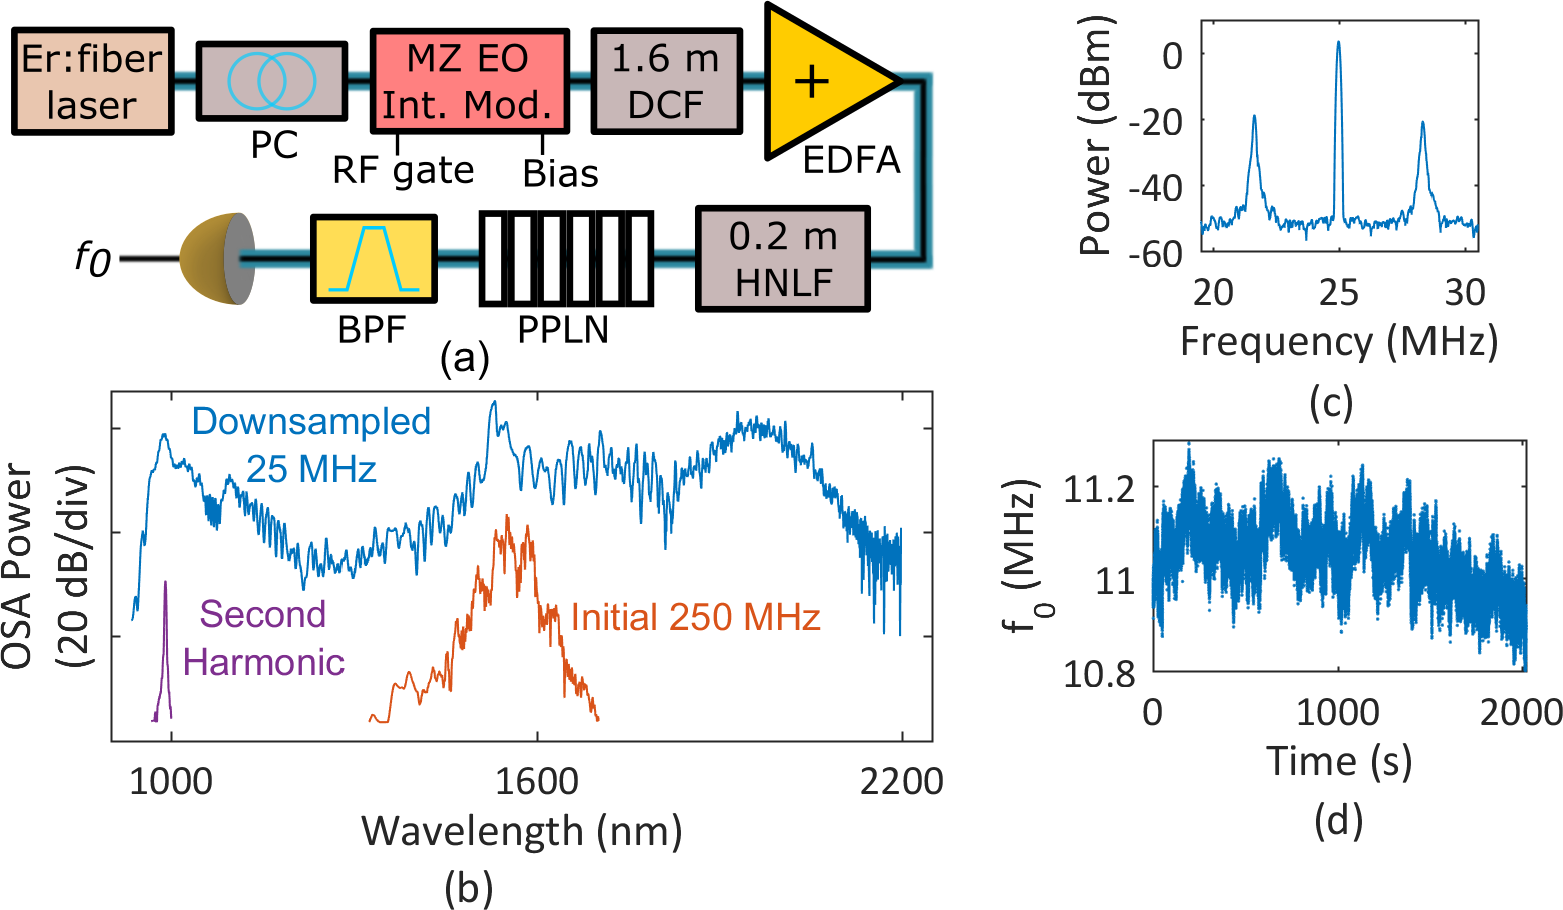
\includegraphics{\FigPath/Figures/PulsePicking/PPProofOfConceptFigv2.png}
	\end{center}
	\caption[Demonstration of downsampling for $f_0$ detection]{\textbf{Demonstration of downsampling for $f_0$ detection.} (a) Schematic depiction of the setup for downsampling a 250 MHz Er:fiber comb and detecting the offset frequency of the resulting 25 MHz pulse train. PC---polarization controller.  DCF---dispersion-compensating fiber. EDFA---erbium-doped fiber amplifier. HNLF---highly nonlinear fiber. PPLN---periodically-poled lithium niobate. BPF---(optical) band-pass filter. (b) Octave-spanning supercontinuum generated by downsampling (top, blue), second harmonic generated for $f_0$ detection (purple), and for comparison the supercontinuum generated by the same apparatus without downsampling (orange). (c) Detected repetition rate and $f_0$ beat at 100 kHz resolution bandwidth; signal-to-noise ratio of $f_0$ is 30 dB. (d) Counted frequency of the detected free-running offset beat. Data is taken for $\sim$2000 s at 10 ms gate time. The offset frequency of the 250 MHz commercial comb was adjusted between measurements shown in Figs. \ref{fig:PPDemo}c and \ref{fig:PPDemo}d to simplify electronic processing.}
	\label{fig:PPDemo}
\end{figure} 



\section{Mathematical model for downsampling}\label{sec:PPMath}
While Fig. \ref{fig:PPDemo} presents an absolute frequency measurement of $f_0$ enabled by downsampling, it does not demonstrate the deterministic connection between the input and downsampled combs that is essential for applications. To understand this relationship, we first consider a simple model of downsampling, and then discuss experimental tests of its conclusions.

The downsampled pulse train's electric field is modeled as the product of the incoming comb's field and a time-varying amplitude modulation. For an incoming optical frequency comb with repetition rate $f_{rep}$, complex single-pulse field $A(t)$ that is localized near $t=0$, and pulse-to-pulse carrier-envelope phase shift $\phi$, pulse gating by a train of rectangular pulses of length $t_g$ and arrival rate $f_g$  yields a downsampled comb with field
\begin{equation}
a(t)=\left[\Sigma_n A(t-n/f_{rep}) e^{in\phi}\right]\times\left[\Sigma_m \mathrm{Rect}\left((t-m/f_g)/t_g \right)\right]  \label{eq:PPmathResult1}
\end{equation}                                            
where $\mathrm{Rect}(x)$ is the rectangle function, taking the value 1 for $-1/2\leq x\leq 1/2$ and 0 elsewhere. Indices $n$ and $m$ count the pulse number of the incoming pulse train and the electronic gate respectively. The optical spectrum of the downsampled pulse train $a(t)$, calculated via the convolution theorem for the Fourier transform, is:
\begin{equation}
\mathcal{F}\{a\}(f)\sim 4\pi f_{rep} \Sigma_{nm}\frac{1}{m}\mathcal{F}\{A\}(f_0+nf_{rep})\times\mathrm{sin}(\pi m t_g f_g)\delta(f-f_0-nf_{rep}-mf_g ),
\end{equation}
where $f_0=f_{rep}\cdot\phi/2\pi$ is the carrier-envelope offset frequency of the incoming comb and $\delta$ is the Dirac delta function.  The downsampled pulse train has spectral content at optical modes $f_0+nf_{rep}$, as well as at intensity modulation sidebands whose frequency offsets $mf_g$ are harmonics of the gating frequency. To avoid the generation of unwanted modulations, pulse gating at an integer sub-harmonic of the incoming repetition rate, $f_g=f_{rep}/N$, is essential. In this case superposition of the intensity modulation components created by pulse gating results in a downsampled frequency comb with a single mode spacing. Moreover, this model predicts that the offset frequency is preserved up to a reduction modulo the comb's new repetition rate. 

Notably, for pulse gating at a sub-harmonic of the input comb's repetition rate, timing jitter of the electronic gate that is less than its duration does not contribute to noise on the downsampled comb. By modeling jitter as gate-to-gate arrival-time delays $\Delta t_m$, it can be shown that the downsampled comb's amplitude $a(t)$ and spectrum $F\{a\}(f)$ do not deviate from Eq. \ref{eq:PPmathResult1} provided that: (1) The jitter is a sufficiently small $|\Delta t_m |<t_g/2$, i.e., that the optical and electronic pulses are always substantially overlapped, and (2) That the optical pulses are substantially shorter than the electrical pulses, which is true for most systems. Thus, in general we expect that the carrier-envelope offset frequency of the incoming comb is preserved by downsampling even with jitter on the gate signal. 

\section{Experimental investigation of the effect of downsampling on the pulse train's noise properties}\label{sec:PPNoiseExp}
We supplement the mathematical model presented above with an experimental investigation of the effects of downsampling on the noise properties of the pulse train. First we consider the effects of technical limitations to ideal downsampling, and then we discuss fundamental effects associated with aliasing of high-Fourier-frequency optical noise and shot noise. 

We measure the phase-noise spectrum of the downsampled comb's repetition rate at different points in our apparatus, as shown in Fig. \ref{fig:PPNoiseExp}a. We also plot the phase noise of the 250 MHz comb, which has been shifted by $-10 \mathrm{log}_{10}(N^2)=-20$ dB to facilitate comparison \cite{Mandridis2010}, and the phase noise of the electronic gate. The downsampled frequency comb's phase-noise spectrum matches that of the 250 MHz comb except for a small increase at $\sim$3 kHz, likely corresponding to the corner in the gate generator's phase noise at the same frequency. The phase noise of the high- and low-frequency ends of the supercontinuum similarly matches the 250 MHz comb below 1 kHz.  The higher phase noise in the supercontinuum beyond 1 kHz is above the measurement system's noise floor (including shot noise), despite the reduced optical power available after spectral filtering. This higher noise is likely due to noise generation processes in the HNLF, such as the conversion of amplitude fluctuations on input pulses to timing jitter in the supercontinuum \cite{Dudley2006}.

\begin{figure}[htpb]
	\begin{center}
		%		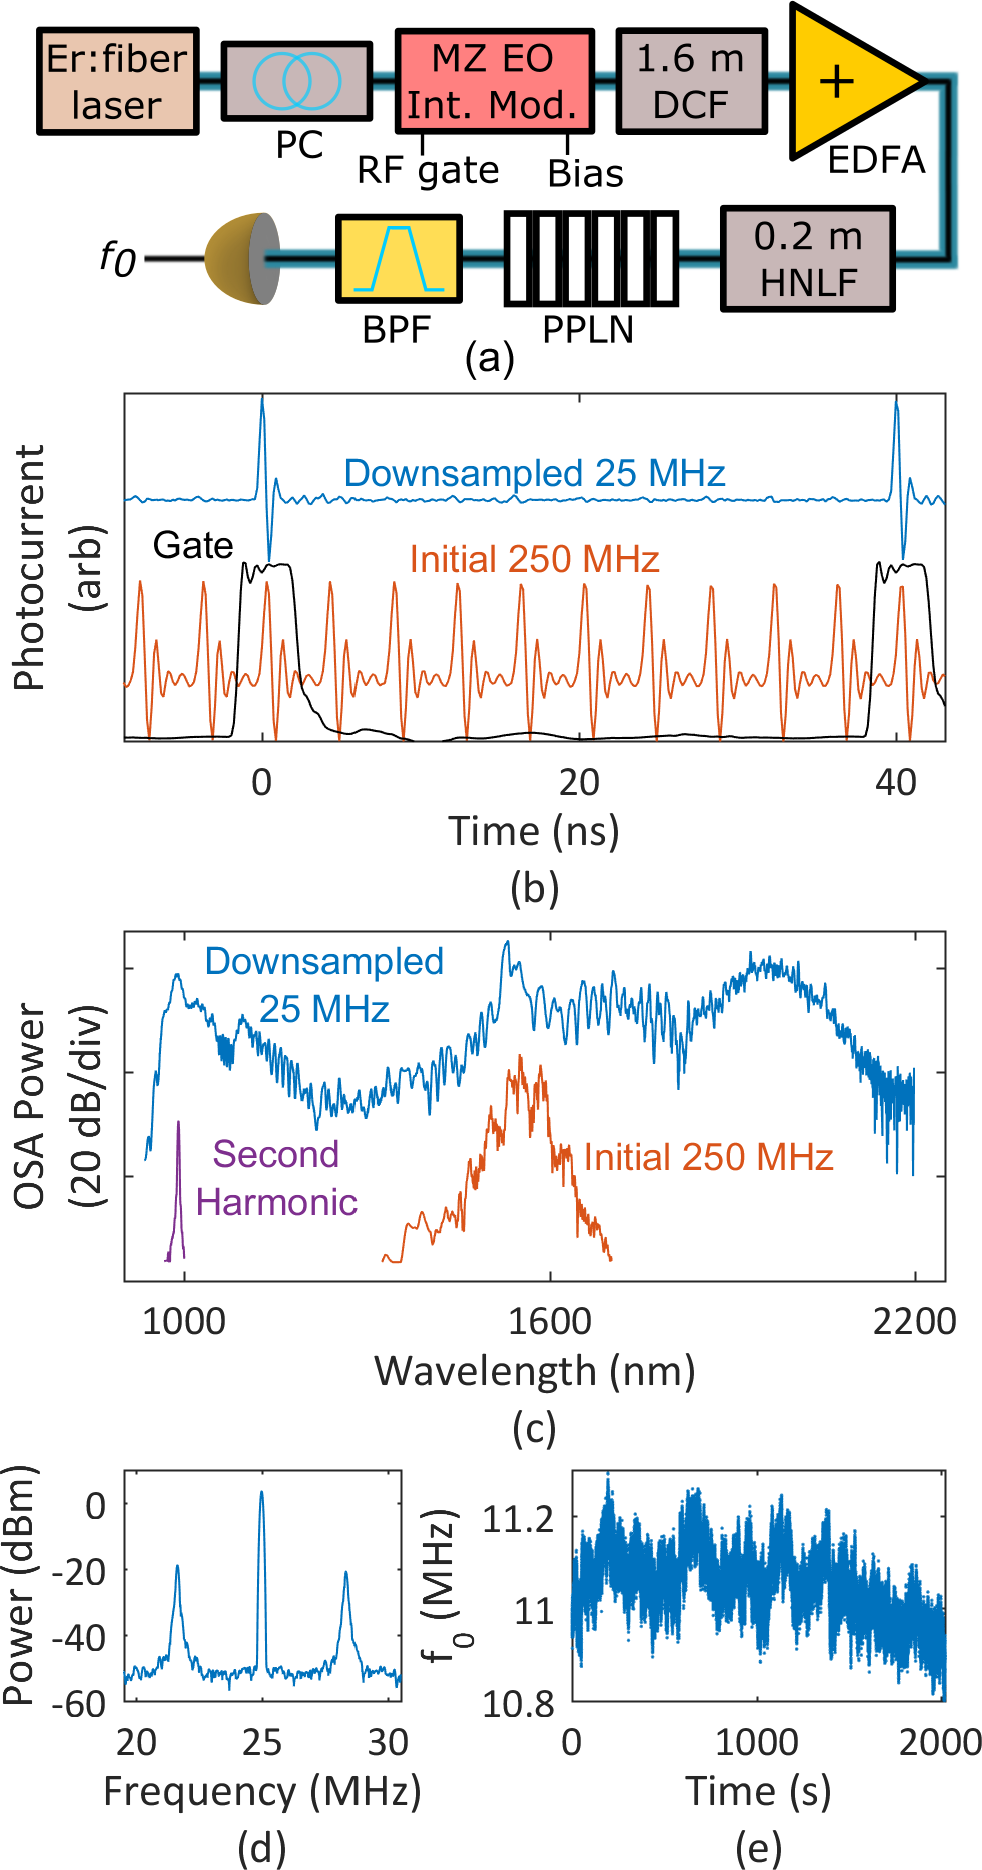
\includegraphics[width=110mm]{\FigPath/Figures/PulsePicking/PulsePickingPaperFig1.png}
		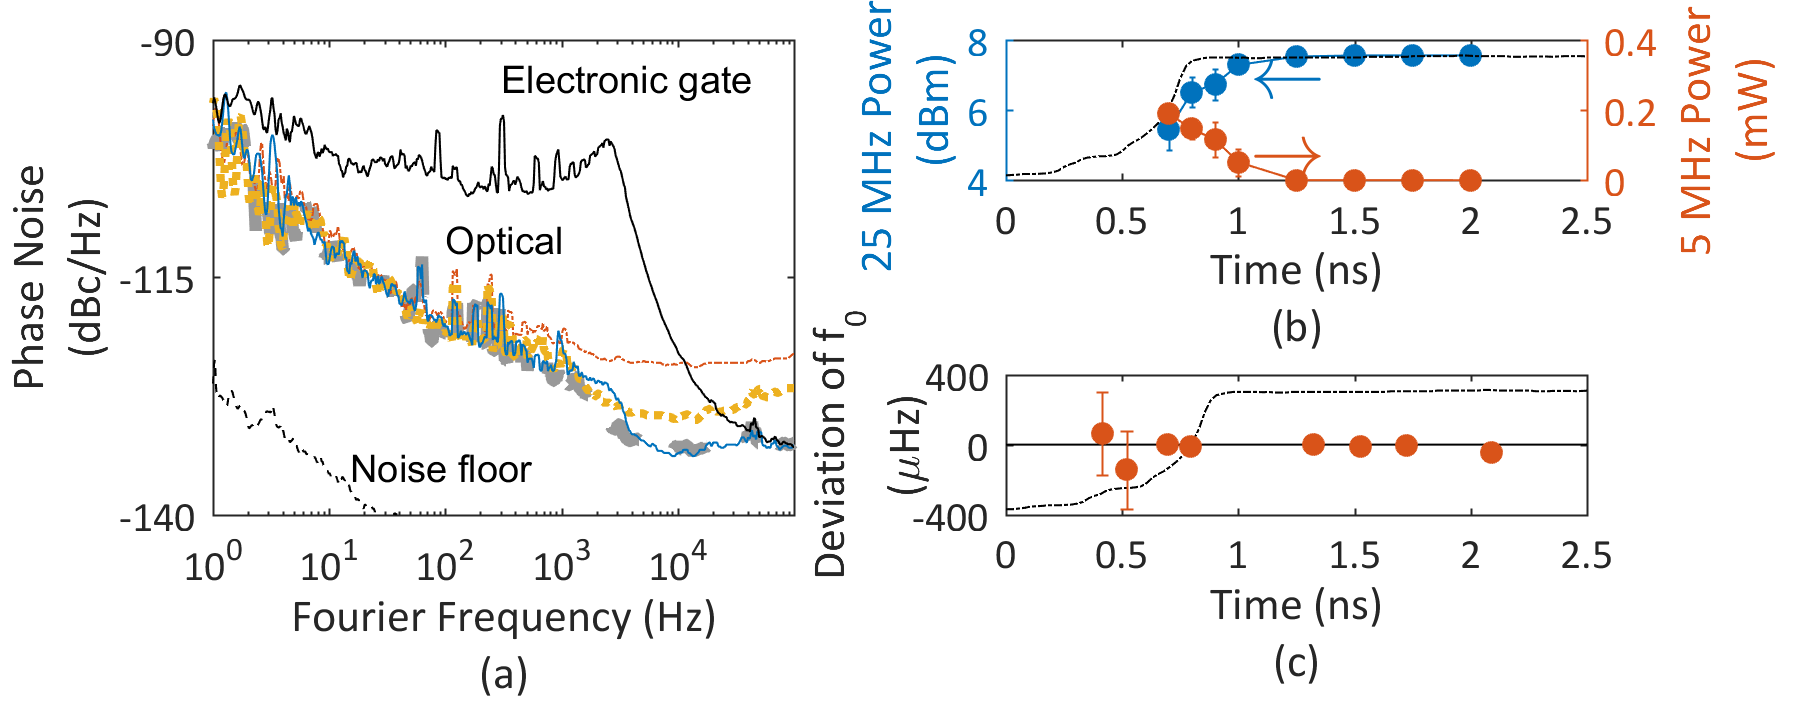
\includegraphics{\FigPath/Figures/PulsePicking/Fig2_thesis.png}
	\end{center}
	\caption[Experimental investigation of noise introduced by downsampling]{\textbf{Experimental investigation of noise introduced by downsampling.} (a) Measured repetition-rate phase noise of spectral components of the supercontinuum, selected by a 990$\pm$5 nm band-pass filter (dot-dashed orange), 1650 nm long pass filter (dotted yellow), and the entire downsampled 25 MHz frequency comb measured immediately before the EDFA (solid blue), the 250 MHz comb (large-dashed gray, shifted by $20\,\mathrm{log}(1/10)=-20$ dB). Also shown is the phase noise of the electronic gate generator (top, solid black). (b) Amplitude of the downsampled pulse-train modulation due to 250 ps jitter at 5 MHz rate. The position of a data point on the x-axis indicates its mean position within the gate, shown in dashed black. Measurement uncertainties arise due to a latency between the optical trigger and the start of the electronic gating signal which varies on the order of 50 ps. (c) Deviation of the carrier-envelope offset frequency of the downsampled comb from the 250 MHz comb's offset frequency as a function of the alignment of optical pulses within the gate.}
	\label{fig:PPNoiseExp}
\end{figure} 

The timing jitter of our gating pulse train is between 5 ps (obtained by integrating the phase noise plotted in Fig. \ref{fig:PPNoiseExp} to 100 kHz) and 10 ps (extrapolating constant phase noise to the 12.5 MHz Nyquist frequency and integrating). These jitter values are small relative to the 4 ns repetition period of the incoming optical pulse train. As the repetition rate of the incoming optical pulse train increases to $>$10 GHz, the gate duration must correspondingly decrease for single-pulse gating, and timing jitter on the gate may become a significant fraction of the gate duration. To explore the effects of timing jitter larger than our pulse generator's inherent 5 to 10 ps, we impose excess jitter on the gating signal. We modulate the relative timing between the gating signal and the incoming optical pulse train at a frequency of 5 MHz with an amplitude of 250 ps. The effect of this jitter is manifest in the microwave power of the gated comb as 5 MHz intensity-modulation sidebands whose amplitude depends on the position of the optical pulses within the gate, as shown in Fig. \ref{fig:PPNoiseExp}b.  Pulses with a mean position within 250 ps of the gate edge are substantially modulated by the 5 MHz gate-delay signal. This agrees with the prediction of a sharp threshold on the acceptable level of timing jitter on the gate.

It is essential to establish that the comb's carrier-envelope offset frequency is preserved in the downsampling process. To do this, we perform a frequency comparison of the 25 MHz downsampled comb and a separate output of the 250 MHz comb. This 250 MHz output is intensity modulated so that a measurement of the nonzero optical heterodyne beat frequency between an intensity modulation sideband and a pulse-gating sideband of the downsampled comb reveals the relative frequency offset of the two combs. Figure \ref{fig:PPNoiseExp}c shows the null frequency shift between the 25 MHz and 250 MHz combs, which we have characterized for different alignments of the optical pulse within the gate. At the level of several microhertz, better than $10^{-18}$ relative to the 200 THz optical carrier frequency, we observe no frequency shift between the 250 MHz comb and the downsampled 25 MHz comb when the gate is properly aligned. This confirms the utility of downsampling for measurement of a high-repetition-rate comb's offset frequency for subsequent use of the comb in, for example, a spectroscopy experiment requiring high power per comb mode and high frequency precision.

\section{Effects of ideal downsampling on a pulse train's noise properties}\label{sec:PPNoiseTheory}

In addition to the conversion of electronic technical noise to optical noise on the downsampled pulse train, there exists a further mechanism by which downsampling can change the measured amplitude noise properties of the pulse train. Even ideal downsampling, free of electronic noise, leads to an increase in the measured power spectral density (PSD) of optical pulse energy fluctuations (PEF) when technical pulse energy noise is present. This is due to aliasing of components of the PSD of pulse energy fluctuations at frequencies above the Nyquist frequency of the downsampled pulse train $f_{rep}/2N$ but below the Nyquist frequency of the original pulse train $f_{rep}/2$. Assuming random fluctuations from pulse to pulse, downsampling does not change the RMS fractional pulse energy fluctuation $\sigma_{PEF}$, whose square is equal to the frequency integral of the PSD of pulse energy fluctuations $S_{PEF} (f)$:
\begin{equation}
\sigma_{PEF}^2=\int_{0}^{f_{rep}/2}df S_{PEF} (f).         
\end{equation}
                       
Because the Nyquist frequency defines the upper limit for integration of $S_{PEF}$, in order for $\sigma_{PEF}$ to be preserved $S_{PEF}(f)$ must increase when the Nyquist frequency is reduced by downsampling. For example, in the simple case of white technical noise on the pulse energies with density $S_o$, we have

\begin{equation}
\sigma_{PEF}^2=\int_{0}^{f_{rep}/2}df S_o=\int_{0}^{f_{rep}/2N}df S^{'}
\end{equation}
which shows that downsampling must increase the measured PSD of white technical noise from $S_o$ to $S^{'}=NS_o$, assuming there are no spectral correlations. However, this simple multiplicative increase is restricted to the case of white technical noise. In general, the PSD of pulse energy fluctuations of the new pulse train is determined from the original PSD through the usual method of modeling aliasing of a signal: a new Fourier frequency for each component of the original PSD is obtained by reducing the original Fourier frequency by a multiple of $-f_{rep}/N$ so that it lies between $-f_{rep}/2N$ and $f_{rep}/2N$ and taking its absolute value. The new PSD is then determined by taking the quadrature sum of the PSD components at the same aliased Fourier frequency. This phenomenon is derived mathematically and demonstrated experimentally in Ref. \cite{Gohle2005}, where the analysis of carrier-envelope phase noise applies equally well to pulse energy fluctuations. 

In contrast with the increase in the PSD of pulse energy fluctuations arising from coincidence of the optical pulse with the edge of the electrical gate, which increases $\sigma_{PEF}$, the aliasing mechanism described above preserves $\sigma_{PEF}$. An important consequence of this is that while technical noise can lead to supercontinuum decoherence in external nonlinear spectral broadening, aliasing does not, because it is $\sigma_{PEF}$ which determines the degree of supercontinuum decoherence. Thus the aliasing mechanism impedes $f-2f$ self-referencing only by reducing the available signal-to-noise ratio of an $f_0$ signal in a straightforward linear fashion. 

In practice, the relevance of the aliasing of the PSD of pulse energy fluctuations is determined by the presence of technical noise on the pulse energies at high Fourier frequency $f > f_{rep}/2N$. For sufficiently small downsampling factors (e.g. $f_{rep}/2N\geq\sim50$ MHz) and depending on the comb source, it is possible that the only source of intensity noise at frequencies above $f_{rep}/2N$ is shot noise. Shot noise results in a maximal (shot-noise-limited) signal-to-noise ratio (SNR) of an optical heterodyne beat with a local oscillator laser which is reduced by $N^2$ (in electrical power units) as the average power of the pulse train is reduced by downsampling by a factor of $N$. In contrast, in the case of detection of a carrier-envelope-offset beat with fixed optical detection bandwidth, the shot-noise-limited SNR is preserved in downsampling. One way to understand these results is to model the shot noise at a given Fourier frequency as the incoherent sum of optical heterodyne beats between each optical comb mode and the uncorrelated vacuum fluctuations at the appropriate optical frequency \cite{Bachor1990,Quinlan2013}, and to take into account the fact that during downsampling the optical power of each comb mode is reduced by $N^2$, with the first factor of $N$ coming from reduction of the total optical power and the second factor of $N$ due to the increase in the spectral density of comb modes. 

We experimentally investigate the impact of downsampling on the PSD of pulse energy fluctuations by measuring noise on three photodetected optical signals: a shot-noise-limited telecommunications-band CW laser, a 10 GHz pulse train generated by passing this laser through cascaded optical phase and intensity modulators (see Chapter \ref{chap:EOMCombs} and Ref. \citeNoBrackets{Cole2016}) and then a low-noise EDFA, and this pulse train after downsampling by a factor of four to 2.5 GHz repetition rate with no additional amplification after downsampling. Shown in Figure \ref{fig:PPSNComparison} are curves for each signal of the fluctuations $\sqrt{S_I (f=50\, \mathrm{MHz})}$ in the detected photocurrent at a Fourier frequency of 50 MHz versus the total time-averaged detected photocurrent $\left<I\right>$ from the optical signal. To measure the scaling of noise with optical power, these curves are generated by beginning with an optical signal that yields more than 800 $\mathrm{\mu}$A of detected photocurrent and attenuating this signal before photodetection. The data indicate that both the pulse-generation process and the downsampling process contribute some amount of technical noise at 50 MHz Fourier frequency to the photocurrent, because the measured curves are well-modeled by a quadrature sum of a shot-noise contribution and a technical noise contribution. The contributions of these two types of noise can be determined because they scale differently with the photodetected power: shot noise obeys the relationship  $\sqrt{S_I (f=50\, \mathrm{MHz})}=\sqrt{2e\left<I\right>}$, $\left<I\right>$ denoting the time-averaged photocurrent, while the technical-noise contribution arises from fluctuations in the expected photocurrent $I(t)$  and scales linearly with the detected photocurrent. We observe that downsampling by a factor of four leads to a multiplication of the amplitude of the technical noise by a factor of $\sim$1.7 on the optical signal relative to the carrier, which due to finite noise bandwidth is somewhat less than the factor of two (four, in electrical power units) that would be expected for ideal downsampling by a factor of four in the presence of white technical noise. These results further demonstrate that, properly implemented, downsampling does not magnify noise on the pulse train to a degree that is prohibitive for applications.

\begin{figure}[htpb]
	\begin{center}
		%		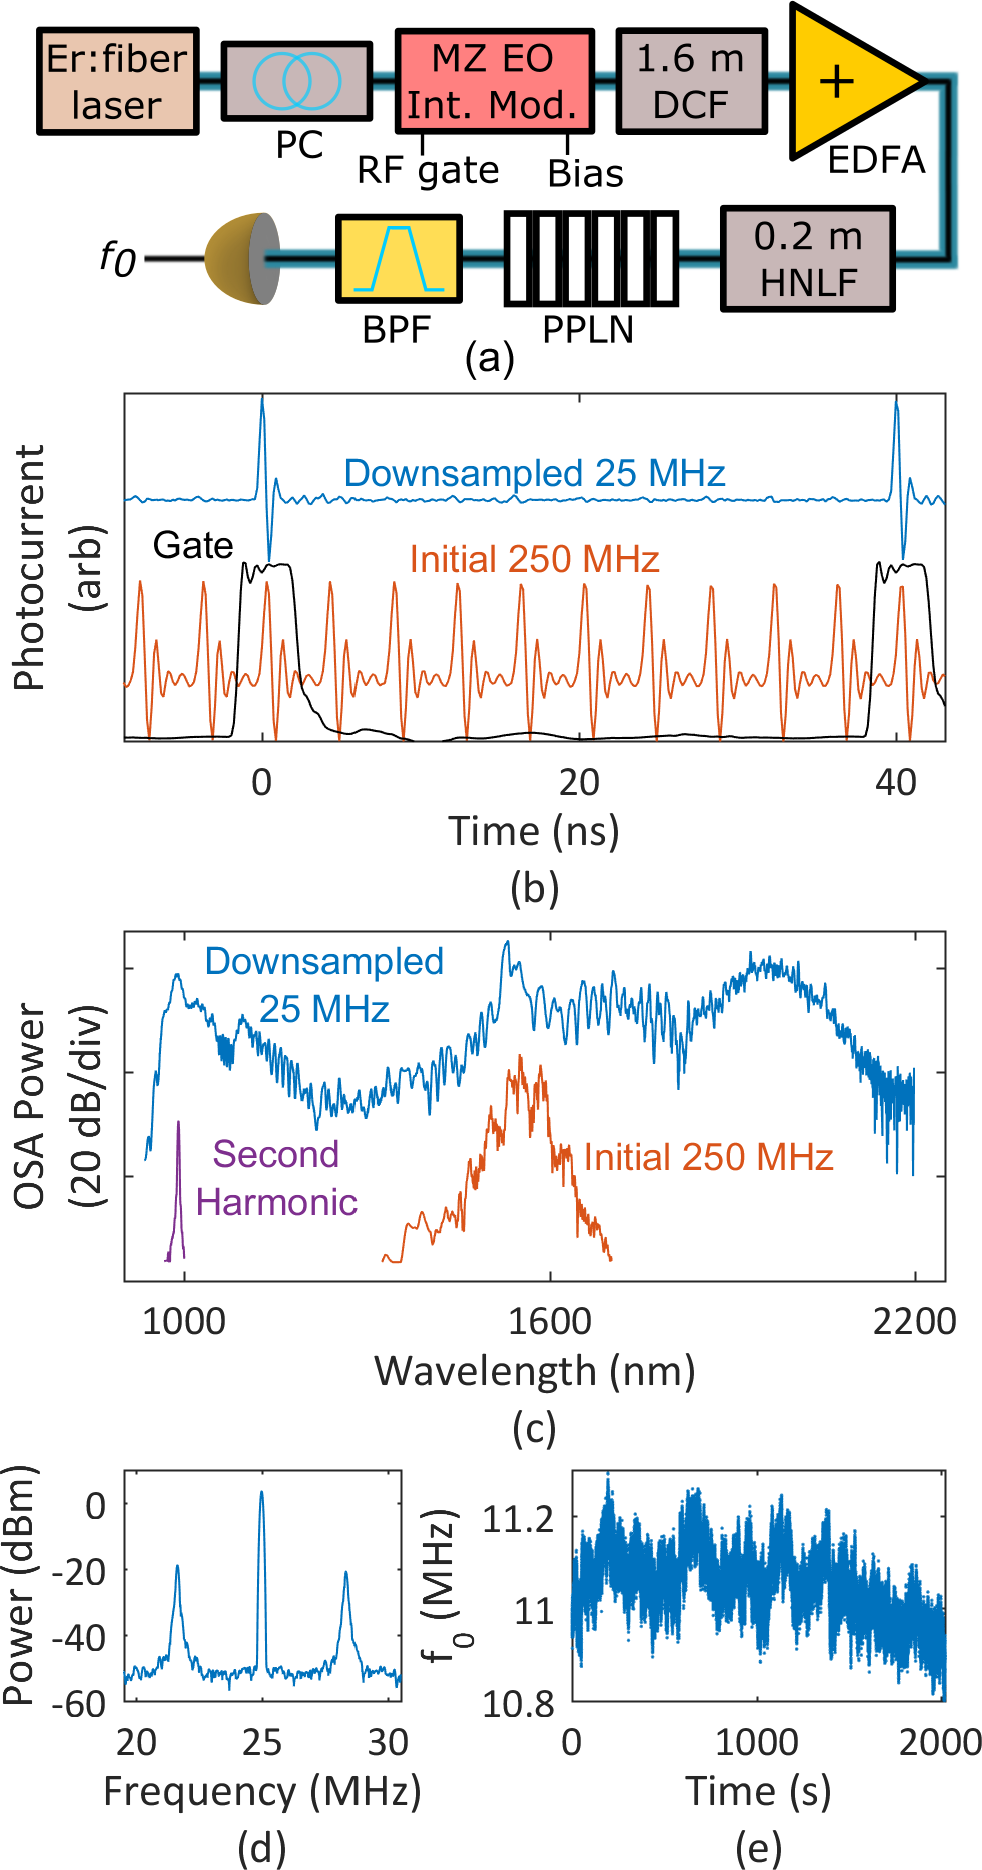
\includegraphics[width=110mm]{\FigPath/Figures/PulsePicking/PulsePickingPaperFig1.png}
		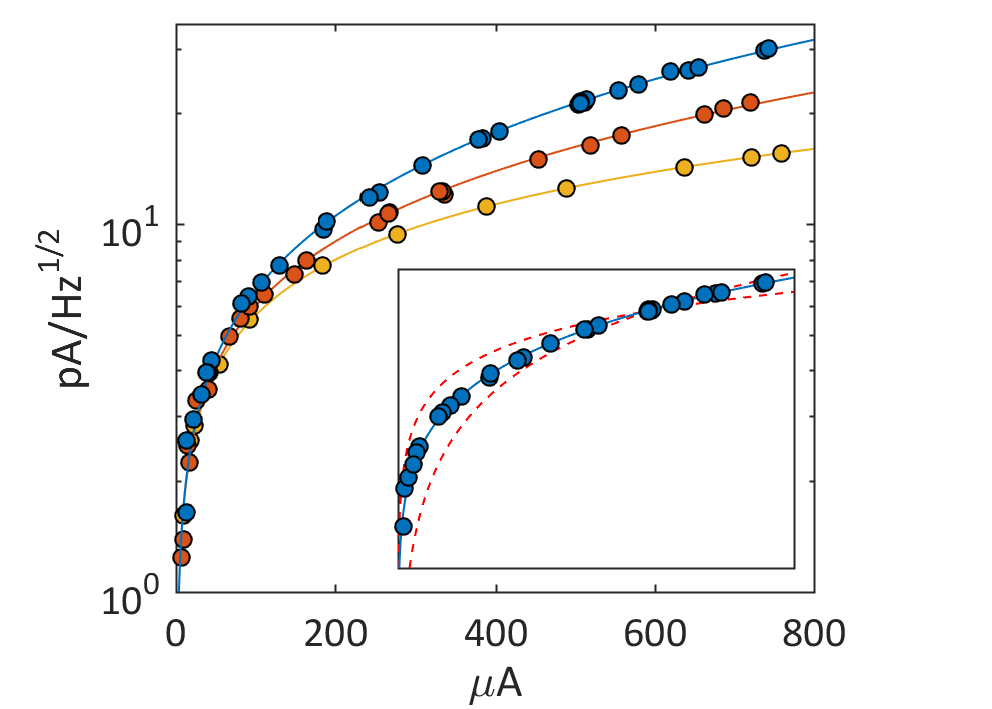
\includegraphics{\FigPath/Figures/PulsePicking/PPSNComparison.png}
	\end{center}
	\caption[Effect of downsampling on photocurrent fluctuations]{\textbf{Effect of downsampling on photocurrent fluctuations.} Fluctuations at 50 MHz Fourier frequency in the detected photocurrent as a function of the time-averaged photocurrent in three cases: CW laser at the shot-noise limit (lowest, yellow), 10 GHz pulse train (middle, red), and 2.5 GHz downsampled pulse train (highest, blue). Dots show measured data and curves show fits to the data. The fit for the shot-noise-limited laser has a single free parameter, which is a scaling factor of order 1 due to frequency dependence of the photodetector's transimpedance gain. The fits for the pulse trains have a scaling factor in common, and have as an additional parameter the amplitude of the technical noise on the pulse train. This is -153.9 dBc/Hz for the 10 GHz pulse train and increases by a factor of $\sim$1.72 to -149.3 dBc/Hz for the 2.5 GHz downsampled pulse train. Inset: Optimized fits (dashed red) to the experimental data for the downsampled 2.5 GHz pulse train using only shot noise or linear technical noise scaling, demonstrating that both noise processes are important for explaining the data. }
	\label{fig:PPSNComparison}
\end{figure} 

\section{Model for the effect of incomplete extinction of rejected pulses and amplification of a downsampled pulse train}\label{sec:PPAmplification}
To this point, we have considered effects of downsampling assuming that extinction of the rejected pulses is complete, but in a practical application this will not necessarily be the case.  The modulators used for pulse extinction may transmit a substantial amount of energy from the rejected pulses---for example, one commercial manufacturer specifies 25 dB extinction ratio, and this number can vary in practice. Additionally, the electronic gating signal may not have sufficient bandwidth to completely switch from transmission to extinction within the repetition period of the incoming pulse train, and initial extinction can be followed by some transmission caused by ringing in the gating signal. Bandwidth limitations will be increasingly likely as the repetition rates of frequency combs increase, placing more demanding requirements on gating electronics.  Incomplete extinction will add modulations to the optical spectrum and will raise the total power of the downsampled pulse train while keeping the energy of the fully-transmitted pulses fixed. This will require higher average power to achieve a given target pulse energy.

The effects of incomplete extinction of rejected pulses are exacerbated if the incomplete extinction does not happen in a deterministic and repetitive fashion; this could occur, for example, if intermediate pulses fall near the edge of the gate in the presence of relative timing jitter between the optical and electronic pulse trains, or if the extinction ratio fluctuates in time. Interestingly, if the downsampled pulse train is subsequently amplified and spectrally broadened, the impact of incomplete extinction depends on whether the optical amplifier used operates in the linear regime or in the saturated regime.

As an example, we consider the case where each fully transmitted pulse is preceded and followed by partially-extinguished pulses whose amplitudes fluctuate for each period of the downsampled pulse train. This fluctuation could occur because the pulses lie on the edge of the electronic gate and there is relative timing jitter between the optical pulse train and the gating signal. It is true that these fluctuations will lead to decoherence during nonlinear spectral broadening. However, the coherence is degraded by this mechanism only within the bandwidth that is achieved by the broadened, partially-extinguished pulses. In efficient $f-2f$ interferometry only the fully-transmitted pulses should reach an octave in bandwidth.  Therefore, this mechanism of supercontinuum decoherence is not a problem in $f-2f$ interferometry in general, unless there is coupling between the amplitudes of the amplified partially-extinguished pulses and the amplified fully-transmitted pulses. This coupling can arise, for example, through amplification in the saturation regime, which then leads to decoherence across the full bandwidth of the supercontinuum. 

To illustrate this point, we have performed numerical simulations of the spectral broadening of a 100 GHz train of 100 fs pulses that has been downsampled to 10 GHz and then amplified. We use an adaptive \cite{Heidt2009} split-step Fourier method \cite{Hult2007} to simulate spectral broadening in 30 cm of HNLF according to the generalized nonlinear Schrodinger equation \cite{Agrawal2007} (see Appendix \ref{app:numericalsims}). In the simulation each fully-transmitted pulse, amplified to 1 nJ, is preceded and followed by partially-extinguished pulses with normally distributed and uncorrelated energies with mean of 0.3 nJ and standard deviation of 0.225 nJ. This models the effect of adjacent pulses that coincide with the edge of the gate. We simulate amplification in two regimes: saturation is simulated using a fixed-energy method wherein the pulse energies in each three-pulse burst are rescaled by a common factor so that the total energy is 1.6 nJ; linear amplification is simulated using a fixed-gain model, which involves no such rescaling of pulses. Numerically, we simulate the spectral broadening of each pulse individually, which is acceptable because terms in the generalized nonlinear Schrodinger equation operate only locally or, in the case of the Raman term, on the timescale of several femtoseconds, while the separation between the pulses in each burst is 10 ps (the inverse of the initial 100 GHz repetition rate).  We have verified that during simulated time-evolution each broadened pulse remains well-centered in its 5 ps simulation window. 

Results of this study are shown in Figure \ref{fig:PPAmp}. Figure \ref{fig:PPAmp}a depicts a three-pulse burst before and after propagation in HNLF. In Figure \ref{fig:PPAmp}b we show spectra corresponding to spectral broadening of this three-pulse burst, as well as plots of the spectral coherence averaged over many simulations. The first-order spectral coherence $g_{12}^{(1)} (\lambda)$ is defined as:
\begin{equation}
\left|g_{12}^{(1)} (\lambda)\right|=\left|\frac{\left<E_1^*(\lambda)E_2(\lambda)\right>}{\sqrt{\left<|E_1(\lambda)|^2\right>\left<|E_2(\lambda)|^2\right>}}\right|=\left|\frac{\left<E_1^*(\lambda)E_2(\lambda)\right>}{\left<|E(\lambda)|^2\right>}\right|.
\end{equation}

Curves are plotted for the fixed-gain and fixed-energy cases, as well as for the case with ideal downsampling (no partially-extinguished pulses) and only shot-noise on the pulse train. The averages in the formula above are over 1000 instantiations of the pair $E_1$ and $E_2$, for a total of 2000 broadened spectra for each pulse within the burst of three. In both the fixed-gain and fixed-energy cases the coherence is poor in the center of the spectrum, but in the fixed-gain case, which models amplification in the linear regime, the coherence is preserved in the high- and low-frequency ends of the spectrum where it is needed for self-referencing.

\begin{figure}[htpb]
	\begin{center}
		%		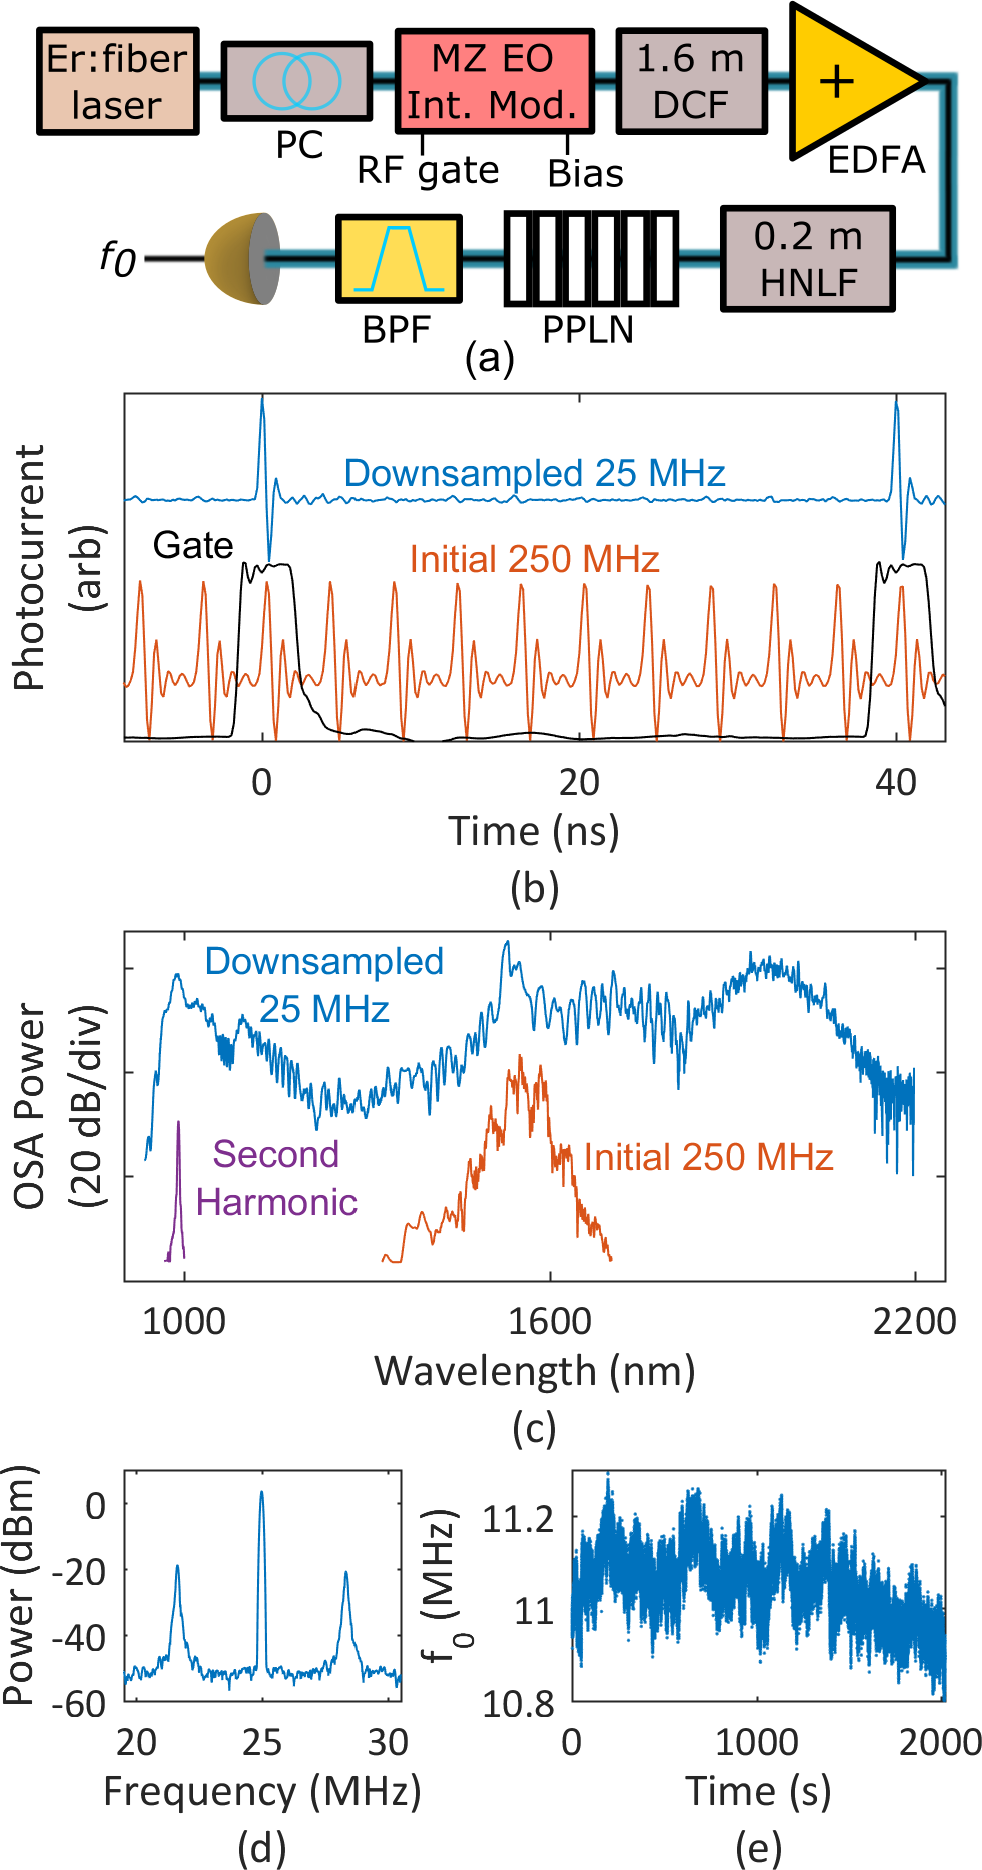
\includegraphics[width=110mm]{\FigPath/Figures/PulsePicking/PulsePickingPaperFig1.png}
		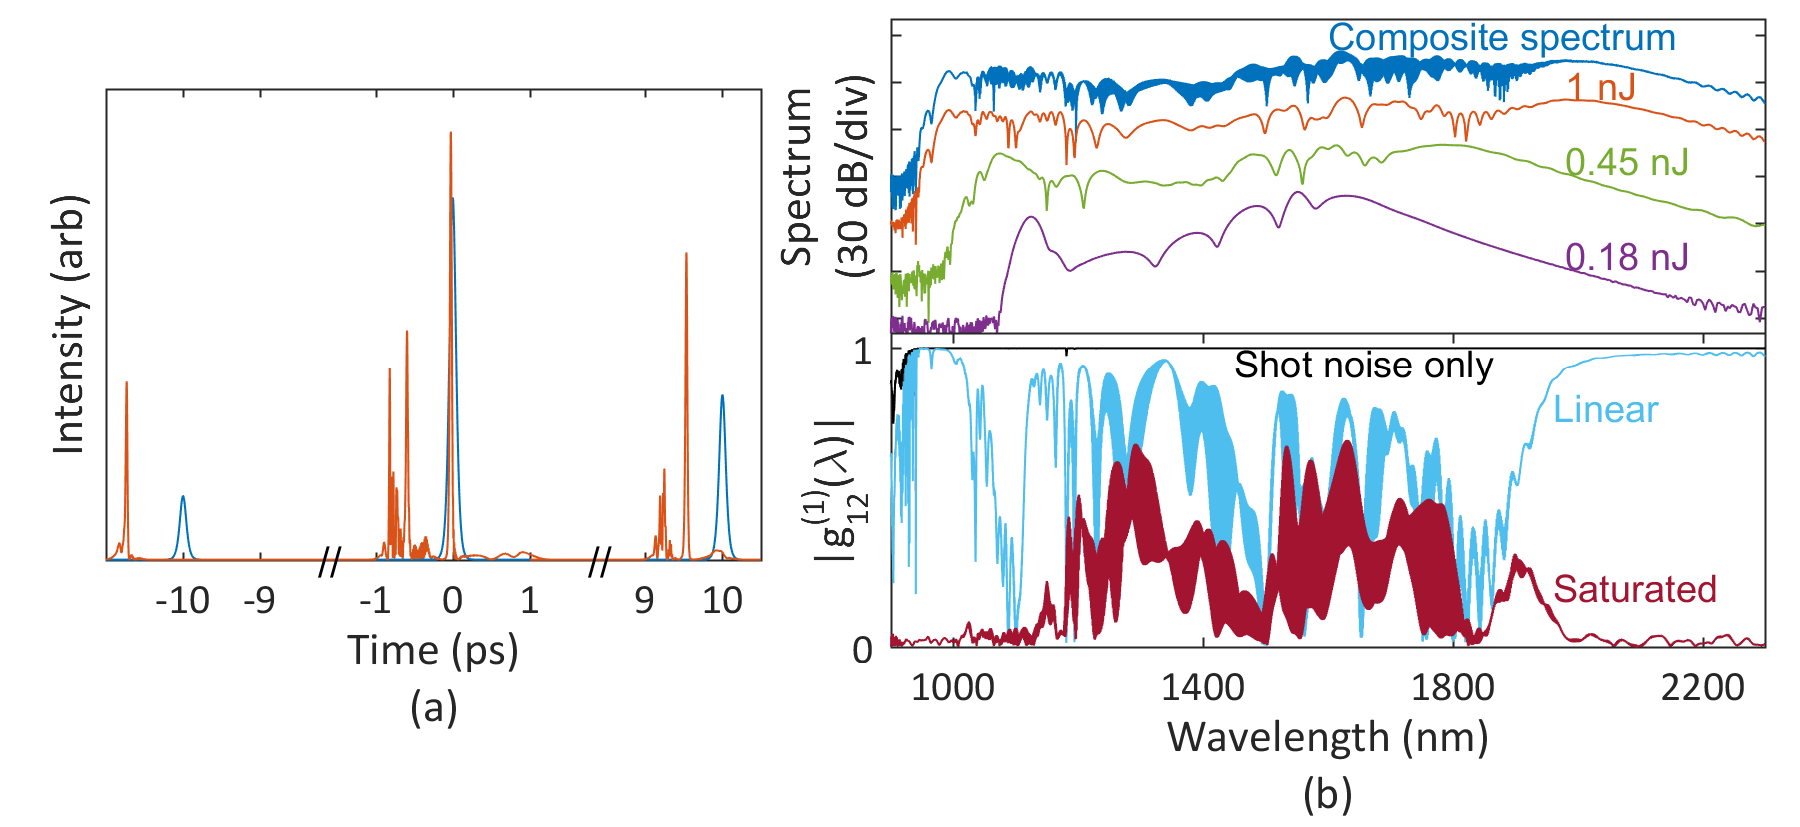
\includegraphics{\FigPath/Figures/PulsePicking/PPAmp.png}
	\end{center}
	\caption[Investigation of incomplete pulse extinction and amplification]{\textbf{Investigation of incomplete pulse extinction and amplification.} (a) A burst consisting of a fully-transmitted 1 nJ, 100 fs pulse and 100 fs partially-transmitted adjacent pulses with energies of 0.18 nJ and 0.45 nJ. Blue indicates initial $\mathrm{sech}^2$ pulses, and orange indicates the intensity after propagation through 30 cm HNLF. Note that the $x$-axis has been broken. (b) Top panel: optical spectra corresponding to the pulses shown in orange in (a), showing the composite spectrum of the three pulses (top, blue) and the spectra of the 1 nJ central pulse (second, orange), the 0.45 nJ adjacent pulse (third, green), and the 0.18 nJ adjacent pulse (bottom, purple). Bottom panel: Calculated spectral coherence averaged over 2000 simulations for the case of shot noise only (top, black) and for the case of fluctuating amplitudes of the first and third pulses as described in the text, after simulated amplification in a linear-regime optical amplifier (second, teal), and a saturated optical amplifier (bottom, maroon).  For the case of linear-regime operation, high spectral coherence is preserved in the extreme ends of the supercontinuum even as it is lost in the center, in contrast with the complete loss of coherence after amplification in saturation. 
	\label{fig:PPAmp}}
\end{figure} 

\section{Further remarks on the application of downsampling}\label{sec:PPConclusion}
Downsampling via pulse gating is a promising tool to manipulate high repetition-rate frequency combs from low size, weight, and power packages and to aid in the detection of their offset frequencies. In our experiments downsampling enabled detection of $f_0$ at a signal-to-noise ratio sufficient for measurement and stabilization, which otherwise would have required significantly higher average power. The effects of the electronic timing jitter of the gate signal are negligible so long as incoming optical pulses do not arrive coincidentally with the edge of the gate; when they do, timing jitter induces amplitude noise on the transmitted pulses. This results in an increase in RMS optical pulse energy fluctuations $\sigma_{PEF}$. Independently, the PSD of pulse energy fluctuations may be increased by aliasing of technical noise and by shot noise, depending on the relative magnitudes of these two types of noise. Each of these sources of signal-to-noise-ratio degradation has the potential to interfere with detection of $f_0$. This investigation of these challenges will facilitate application of the technique in high repetition-rate frequency comb systems. Importantly, our experiments demonstrated that downsampling does not add a significant amount of noise to the frequency components of the pulse train, and in a separate experiment the technique has recently been used successfully to detect the carrier-envelope offset frequency of a 10 GHz comb by downsampling by a factor of four (\cite{Beha2017}, see Chapter \ref{chap:EOMCombs}).

To employ downsampling as demonstrated here with repetition rates $>$10 GHz will require electronic gates with duration $\leq$100 ps. Technology to downsample with gates as short as 20 ps is commercially available, while 100 Gb$/$s integrated circuits and 25 GHz demultiplexing have been demonstrated \cite{Driad2011,Ferenci2012}, and this technology continues to improve. Barring the use of such state-of-the-art electronics, pulse gates of duration longer than the incoming optical pulse train's repetition period can be employed.  This will be technically easier to achieve, but will result in additional modulations on the spectrum of the downsampled pulse train.

The ambiguity of the input comb's offset frequency as a result of the reduction of the offset frequency modulo the new repetition rate makes downsampling most suitable for applications where the ambiguity can be removed by some other method.  Two such applications are frequency comb calibration of astronomical spectrographs, where measurement of the wavelength of a comb mode can remove the ambiguity, and microresonator-based frequency combs, where the uncertainty in the offset frequency is determined by the frequency stability of the pump laser and can be much less than the repetition rate of the downsampled comb. 





% \chapter{Microresonator-based frequency combs: Summary and outlook}\label{chap:conclusion}

Chapters \ref{chap:microresonators}-\ref{chap:FPLLE} discussed generation of frequency combs from a continuous-wave laser by parametric frequecy conversion in Kerr-nonlinear resonators. I described three results: 1. The investigation and implementation of a technique for spontaneous soliton generation in Kerr resonators using a phase-modulated pump laser, 2. The observation and explanation of soliton crystals in Kerr resonators, and 3. A theoretical investigation of Kerr-comb generation in Fabry-Perot cavities, with an emphasis on the properties of solitons and soliton generation. These results all help to more clearly define what is possible with these systems, and suggest avenues for further research. 

Soliton generation with a phase-modulated pump laser is a promising candidate for inclusion in chip-integrated Kerr-comb systems as the mechanism by which single-soliton operation is initiated. Two directions for continued work are additional theoretical investigations of the full LLE with a phase-modulated pump, which could provide insight into the dynamics beyond what is possible using the approximations described in Chapter \ref{chap:PMpumping}; and implementation of the technique with resonators that have electronically-inaccessible free-spectral ranges, using the subharmonic-modulation approach that was proposed. Incorporation of the technique into a chip-integrated Kerr-soliton comb may also require modification and further devleopment of the technique that was used to overcome thermal instabilities associated with the increasing-frequency pump-laser scan.

The investigation of soliton crystals presented here serves several important purposes. First, it represented an important step towards full explanation of observed Kerr-comb phenomena in terms of the LLE model. \todo{am I citing pascal in sc chapter?} Second, soliton crystals have the attractive properties of single-soliton Kerr combs, with the additional property that a soliton crystal of $N$ pulses has conversion efficiency of pump-laser power into the comb that is roughly $N$ times higher than a comparable single-soliton comb. With careful preparation of a particular crystal state, this could make them attractive for applications like optical arbitrary waveform generation and nonlinear spectroscopy. Additionally, soliton crystals present a hugely degenerate configuration space that could be useful in implementations, for example, of an on-chip optical buffer or in communications applications \cite{Leo2010a}. Finally, experimental generation of soliton crystals is significantly simpler than generation of single solitons, where the change in the duty cycle of the optical waveform from extended pattern to single soliton leads to thermal instabilities that are alleviated only with precise control of the pump-laser power and frequency. Thus, it is possible to propose a scheme for deterministic on-chip soliton crystal generation that makes use of two resonators, each constructed of looped single-mode optical waveguides. One resonator is pumped by a laser and hosts the soliton crystal. The second resonator need not be pumped, and exists to provide a specific perturbation to the mode structure of the first resonator to enable soliton crystallization; this could be achieved through careful engineering of the coupling between the resonators. If the free-spectral range of the second resonator is considerably higher than the free-spectral range of the first, and not near one of its harmonics, then realization of single-mode perturbation to the mode structure of the first resonator could be achieved. Implementing deterministic soliton crystal generation on a chip in this way could greatly simplify requirements on the other components in a system for full-integration of Kerr solitons, as soliton generation could be achieved through slow tuning of the pump laser.

The theoretical investigation of Kerr-comb generation in the Fabry-Perot geometry will provide useful guidance for future experimental work. An obvious direction for continued work is the generation of solitons in Fabry-Perot cavities that make use of the additional degree of freedom provided by the dispersion applied by reflection at the ends of the cavity. This would build on previous experiments \cite{Braje2009,Obrzud2017}. In fact, soliton generation in Fabry-Perot cavities constructed of potted fiber ferrules with high-reflectivity end-coatings has already been realized at NIST Boulder \cite{Zhang2018}, but there remains work to be done to achieve control the total cavity dispersion with chirped mirror-coatings. Unresolved questions include the effect of uncontrolled expansion of the mode in the coating on both the mirror reflectivity and its group-velocity disperson. Looking to the chip scale, integrated Fabry-Perot cavities constructued of single-mode waveguides with photonic-crystal mirrors is a promising route for development that would further reduce the footprint of Kerr-comb systems. This work is ongoing at NIST Boulder, and primary comb has been observed in such a cavity \cite{Yu2018}. Finally, I note that the proposal for deterministic chip-scale generation of soliton crystals presented above could be realized with two co-linear on-chip Fabry-Perot cavities, where the first cavity hosts the crystal, which is out-coupled in reflection, and the second cavity provides a perturbation to the first cavity's mode structure.







 
\appendix
%\include{AppendixATI}
%\include{AppendixPEI}
%\include{AppendixShock}

\begin{spacing}{1.3}
\printbibliography[heading=bibintoc,title={References}]
\end{spacing}

\end{document}
